\documentclass[tocnopagenum]{thesis-ekf}
%a4paper, 12pt, 1.5-es sortávolság, margók
\usepackage[T1]{fontenc}
\PassOptionsToPackage{defaults=hu-min}{magyar.ldf}
\usepackage[magyar]{babel}
\usepackage{mathtools,amssymb,amsthm,pdfpages}
\footnotestyle{rule=fourth}
\usepackage{comment}
\usepackage{enumitem}
\usepackage{colortbl}
\newtheorem{tetel}{Tétel}[chapter]
\theoremstyle{definition}
\newtheorem{definicio}[tetel]{Definíció}
\theoremstyle{remark}
\newtheorem{megjegyzes}[tetel]{Megjegyzés}
\graphicspath{{./images/}}
\DeclareGraphicsExtensions{.png,.jpg,.pdf}
%excel to latex
\usepackage{booktabs}
\usepackage{bigstrut}

%algorithm
\usepackage{algorithm}
\usepackage{algpseudocode}


\begin{document}
	\institute{Matematikai és Informatikai Intézet}
	\title{Informatikai eszközökkel támogatott sport és egészségfejlesztés}
	\author{Sipos Levente\\Szak: Programtervező informatikus BSc\\Specializáció: Szoftverfejlesztő informatikus}
	\supervisor{Dr. Király Roland\\docens}
	\city{Eger}
	\date{2022}
	\begin{titlepage}
		\maketitle
	\end{titlepage}
	
	\tableofcontents

	\addcontentsline{toc}{chapter}{Bevezetés}
	\addcontentsline{toc}{chapter}{Elméleti háttér}
	\addcontentsline{toc}{chapter}{Összegzés}



	\begin{comment}
		leírom hogy miről szól, (nem kötelező), 2 rész -> probléma felvetés, mi a motiváció, kontextus, előremutatva a dolgozatban hol miről fogsz beszélni.(1.fejezetben befogom mutatni a kódolást)
	\end{comment}
	\chapter{Bevezetés}

	A tanulmányaim során sok olyan tárgyat tanulhattam amelyek segítettek belátást nyerni, hogy valójában melyik is az az irányágazat az informatikán belül, amely felkeltette az érdeklődésemet. Az utolsó félévekben tanulhattam robotikát a Robotika alapjai nevezetű tárgy következtében, amely közelebb vitt engem a gépközeli programozás világába. Továbbá C\# nyelvben elég biztos tudást szerezhettem a Szolgáltatás Orientált Programozás, Magasszintű programozási nyelvek I. és II. című tárgyakon.
	\par
	Szakdolgozatom tematikájául szerettem volna egy olyan témát választani, melynek a későbbiekben másoknak tudok segítséget nyújtani az informatikai szaktudásommal.
	Mint keresztény hívő ember, úgy gondolom, hogy az emberi létünk egyik fő feladat és mozgatórúgója az az, hogy segítsünk embertársainkon azokkal a technikákkal és tudásokkal amelyek számunkra megadattak. Ezért örömmel tölt el az a lehetőség, hogy tanulmányaimat ennek a segítségére fordíthatom. 
	\par
	A választott téma, mind az informatika mind, az egészségügy számára fontos kérdéseket tehet fel:
	\begin{itemize}
		\item  Mi jelenthet arra megoldást, ha egy adott korosztályba tartozó ember, nehézségekkel küzd a mindennapokban, a mozgását, illetve a mentális felfogását illetően? (Akár ez jelentheti az egyszerű mozgások nem megfelelő elvégzését, akár pedig az alap információk felfogásában való akadályozottságot is.)
		\item  Az informatikával tudunk-e az előbb említett kérdésre, olyan alkalmazást írni, amely ezeknek a fejlődését elősegítheti?
		\item A testnevelés tudomány és a technika az informatikával társítva, hogyan tudja segíteni az emberi mozgást?
		\item Amennyiben tudunk ilyen alkalmazást írni, hogyan valósítsuk meg?
	
	\end{itemize}
 	Ezen kérdések alapján keresem a válaszokat arra nézve, hogy az informatika hogyan tud segítségére lenni a fizikai létnek. 
 
	Meglátásom szerint, ez egy hiánypótló kutatási téma, amely az embereknek a mozgását, és fizikai jólétét segítheti elő.
	Ezen eszközök leptikus területeket érintenek, vizuális illetve akusztikus hatások közreműködésével.
	\\
	A projekt fontossága az, hogy ezen eszközök segítséget tudjanak nyújtani, esetleg kiváltsák a beszédnek a szolgálatát. Ahol már beszéd nem elegendő ott ezen eszközök segíthetik a mozgásában fejlődésre szoruló egyéneket. Mind a fiatalok mind a szépkorúak számára hasznos gyakorlat lehet.
	\\ 
	A digitális fejlődéssel egyre több eszköz segíti az arra rászorulókat, például a mostanság kutatásban lévő gondosóra, program amely a szociális segítésben vesz részt az idősgondozásban.\cite{MTI}
	\\
	A cél az embereknek a fizikai illetve mentális állapotának elősegítése.
	\par 
	
	Alapvetően a következő fejezetekben azt szeretném részletezni, hogy milyen technológiákat használunk, és emellett milyen programozási nyelven készül a projekt. \\ 
	Továbbá, ki fogok térni azokra a rendszerekre is, amelyek hasonló céllal készültek el. Majd ezen projekteket hasonlóságait és különbségeit mérném össze, az elkészült projektünkkel. 
	
	\begin{comment}
	Bevezető2: Rendszer amit kidolgozott Somodi László, mi a szerepe, mi a célja, mit vállaltam én? -> frontend
	\end{comment}
	\chapter*{Háttérelmélet}
	\par
	A témában jártas, és a "Mozgáskoordináció- és gyorsaságfejlesztő gyakorlatok óvodától a felnőtt korig" \cite{SLaszlo} című könyv írója, Somodi László, segített belátást nyerni az egészségügyi és a morális lényegességébe a projektnek. \\ Elmondása szerint a mozgásfejlesztés és az agyi kapacitás fejlesztése, kéz a kézben jár. Ezt a mozgásfejlesztést úgy érhetjük el, ha az adott személynek utasításokat adunk ki, hogy adott jelzésre (szín, hang, irány) és ezek kombinációjára, milyen mozgást kell végeznie.
	\par 
	\subsection*{Gyakorlati haszna}
	Az agy mentális funkcióinak erősítése, speciális koordinációfejlesztő gyakorlatokkal is lehetséges melynek a három komponense a következő: 
	\begin{enumerate}
	 
			\item	Az első komponens a koncepció, vagyis az a módszer, ami alapján a rendszer elkészült. A koncepció egészségügyi, és sport-rekreációs tevékenység alapú.
			\item	A második komponens a hardver, ami a mozgáshoz és a gyakorláshoz szükséges időzítést, jelzéseket adja, és vezérli az aktivitást, amit a koncepció előír.
			\item	A harmadik komponens a hardvert meghajtó, és így a feladatokat közvetlenül irányító, programozható, tanítható szoftver.
	\end{enumerate}
	\subsection*{Módszer lényege}
	Az a személy aki használja ezt, nála külön dolgozik a két kar, külön dolgozik a két láb és ezáltal folyamatosan kapcsoljuk át a két agyféltekét.
	Továbbá, a könnyen és egyszerűen felismerhető hang, szín, és ábra jelzések az esetlegesen a fogyatékossággal élő emberek számára se jelenthet akadályt.
	\\
	Különféle álló helyzetek (alapállás, mellső középtartás, magas tartás) képesek segíteni abban, hogy az idegpályákon lévő átkapcsolódási pontok (szinapszisok) száma növekedjen. Fiatalabb korban a szinapszisok számát, későbbiekben az átkapcsolódási pontok erejét növeli.
	Sokféle betegség felmerülhet az olyan embereknél akiknek ez a módszer alkalmas lehet, a könnyen felismerhető és megérthető eszközök.
	Továbbá, ez által a módszer által gyorsabban megértjük az elvégzendő  feladatot, feladatokat és akár gyorsabban is végrehajthatjuk azokat.
	  %szellemi leépüléssel küzdő, szép korúak számára is segítséget nyújthat, mivel a változatos mozgás, és a különböző ingerek ki- és be- kapcsolása növeli az agy alap működését.
	 \\
	Gyakorlati tapasztalatunk szerint a módszer hasznosan alkalmazható általános helyzetű, HH és HHH helyzetű és beteg gyerekeknél is. Kutatásaink és mért eredményeink ezt támasztják alá.
	A módszert kis helyen és minden korosztálynál lehet alkalmazni, de a teljesség érdekében, a módszer intelligens szobával együtt működik hatékonyan.
	
	
	\subsection*{Intelligens szoba röviden}
	Az intelligens szoba kifejezés egy olyan helység, melynek mind a négy falán, vagy oldalán különböző jeladókat helyezünk el.
	Ezek különböző eszközök melyek típusai lehetnek: fények, színek, nyilak és hangok. Ezek külön, vagy együttesen kiküldött jeleire különböző, illetve speciális koordinációfejlesztő feladatokat végrehajtani. Minden egyes különböző szín, és fényjelzés, más és más feladatokat tartalmaznak.
	Ez azt jelenti, hogy adott esetben egy piros lámpa színe emlékeztethet arra, hogy a piros szín jelentése szimbolikus hatással bír.Melyet az adott ember köthet a már mindennapos életben tapasztaltakhoz. Nyilak felvillanására, különböző hangokra pedig más érzékeket váltunk ki mint például a fényjelzés esetén. Ilyenkor irányváltásokat kell végrehajtani amik máris komplikálják egy kicsit az adott mozdulatokat.
	\\
	Ezzel a módszerrel és az intelligens szobával együttesen tudjuk a mozgáson keresztül úgy stimulálni az agyat, hogy a legrövidebb idő alatt a legtöbbször átkapcsoljuk. ( 200-szor, 300-szor, 400-szor, stb. )
	\par
	\subsection*{Automatizálás célja}
	A fentebb említettek automatizálására készül a projekt, amely különböző informatikai eszközökkel valósítja meg a színek, hangok, és nyilak megjelenítését, illetve érzékeltetését. 
	A hardver komponensek. A hardver több egymáshoz tetszőlegesen kapcsolható smart box, amelyek képesek fényjelzések, fénnyel képzett ábrák, valamint hangjelzések kiadására. A smart box-okat szoftveresen lehet vezérelni, így azok képesek a koncepció alapján összetett mozgások, vagy komplex feladatsorok irányítására.
	Ennek egy példája a \pageref{table:egyedzesterv}. oldalon található táblázat amely az automatizálásra létrehozott "edzéstervet" mutat be.[\ref{table:egyedzesterv}]
	\begin{table}[h]
		\centering
		\caption{Egy adott edzésterv}
		\scalebox{0.7}
		{
			\begin{tabular}{|rrrrlrrrrr|}
				\hline
				\multicolumn{1}{|l|}{\textbf{helyzet}} & \multicolumn{1}{l|}{\textbf{egység típusa}} & \multicolumn{1}{l|}{\textbf{jel száma}} & \multicolumn{1}{l|}{\textbf{szín}} & \multicolumn{1}{l|}{\textbf{hang}} & \multicolumn{1}{l|}{\textbf{irány}} &       &       & \multicolumn{1}{l}{\textbf{fenntartási idő}} & \multicolumn{1}{l|}{\textbf{irány}} \bigstrut\\
				\hline
				&       &       &       &       &       &       &       &       &  \bigstrut[t]\\
				&       &       &       &       &       &       &       &       &  \\
				\multicolumn{1}{|c}{1} & \multicolumn{1}{c}{2} & \multicolumn{1}{c}{3} & \multicolumn{1}{c}{4} & \multicolumn{1}{c}{5} & \multicolumn{1}{c}{6} & \multicolumn{1}{c}{7} & \multicolumn{1}{c}{8} &       &  \\
				\multicolumn{1}{|c}{lámpa} & \multicolumn{1}{c}{lámpa} & \multicolumn{1}{c}{hang} & \multicolumn{1}{c}{lámpa} & \multicolumn{1}{c}{nyíl} & \multicolumn{1}{c}{lámpa} & \multicolumn{1}{c}{lámpa} & \multicolumn{1}{c}{nyíl} &       &  \\
				&       &       &       &       &       &       &       &       &  \\
				\multicolumn{1}{|l}{szemben} &       &       &       &       &       &       &       &       &  \bigstrut[b]\\
				\cline{1-2}\cline{7-7}    \rowcolor[rgb]{ .6,  .8,  0} \multicolumn{1}{|c|}{\textcolor[rgb]{ .2,  .6,  .4}{zöld}} & \multicolumn{1}{c|}{\cellcolor[rgb]{ 1,  0,  0}piros} & \cellcolor[rgb]{ 1,  1,  1} & \multicolumn{1}{c}{\cellcolor[rgb]{ 1,  1,  0}sárga} & \cellcolor[rgb]{ 1,  1,  1} & \multicolumn{1}{c|}{\cellcolor[rgb]{ .2,  .4,  1}kék} & \multicolumn{1}{l|}{\cellcolor[rgb]{ 1,  1,  1}fehér} & \cellcolor[rgb]{ 1,  1,  1} & \cellcolor[rgb]{ 1,  1,  1} & \cellcolor[rgb]{ 1,  1,  1} \bigstrut\\
				\cline{1-2}\cline{7-7}    \rowcolor[rgb]{ 0,  0,  0}       &       &       &       &       &       &       &       &       &  \bigstrut\\
				\cline{2-2}    \multicolumn{1}{|r|}{} & \multicolumn{1}{c|}{\cellcolor[rgb]{ 1,  0,  0}1 piros} &       &       &       &       &       &       & \multicolumn{1}{c}{16"} &  \bigstrut\\
				\cline{2-2}\cline{4-4}          &       & \multicolumn{1}{c|}{} & \multicolumn{1}{c|}{\cellcolor[rgb]{ 1,  1,  0}2 sárga} &       &       &       &       & \multicolumn{1}{c}{1"} &  \bigstrut[t]\\
				&       & \multicolumn{1}{c|}{} & \multicolumn{1}{c|}{\cellcolor[rgb]{ 1,  1,  0}2 sárga} &       &       &       &       & \multicolumn{1}{c}{16"} &  \bigstrut[b]\\
				\cline{1-1}\cline{4-4}    \rowcolor[rgb]{ .6,  .8,  0} \multicolumn{1}{|c|}{1 zöld} & \cellcolor[rgb]{ 1,  1,  1} & \cellcolor[rgb]{ 1,  1,  1} & \cellcolor[rgb]{ 1,  1,  1} & \cellcolor[rgb]{ 1,  1,  1} & \cellcolor[rgb]{ 1,  1,  1} & \cellcolor[rgb]{ 1,  1,  1} & \cellcolor[rgb]{ 1,  1,  1} & \multicolumn{1}{c}{\cellcolor[rgb]{ 1,  1,  1}1"} & \cellcolor[rgb]{ 1,  1,  1} \bigstrut[t]\\
				\rowcolor[rgb]{ .6,  .8,  0} \multicolumn{1}{|c|}{1 zöld} & \cellcolor[rgb]{ 1,  1,  1} & \cellcolor[rgb]{ 1,  1,  1} & \cellcolor[rgb]{ 1,  1,  1} & \cellcolor[rgb]{ 1,  1,  1} & \cellcolor[rgb]{ 1,  1,  1} & \cellcolor[rgb]{ 1,  1,  1} & \cellcolor[rgb]{ 1,  1,  1} & \multicolumn{1}{c}{\cellcolor[rgb]{ 1,  1,  1}16"} & \cellcolor[rgb]{ 1,  1,  1} \bigstrut[b]\\
				\cline{1-1}\cline{6-6}          &       &       &       & \multicolumn{1}{c|}{} & \multicolumn{1}{c|}{\cellcolor[rgb]{ .2,  .4,  1}1 kék} &       &       & \multicolumn{1}{c}{1"} &  \bigstrut[t]\\
				&       &       &       & \multicolumn{1}{c|}{} & \multicolumn{1}{c|}{\cellcolor[rgb]{ .2,  .4,  1}1 kék} &       &       & \multicolumn{1}{c}{8"} &  \bigstrut[b]\\
				\cline{4-4}\cline{6-6}          &       & \multicolumn{1}{r|}{} & \multicolumn{1}{c|}{\cellcolor[rgb]{ 1,  1,  0}2 sárga} &       &       &       &       & \multicolumn{1}{c}{1"} &  \bigstrut[t]\\
				&       & \multicolumn{1}{r|}{} & \multicolumn{1}{c|}{\cellcolor[rgb]{ 1,  1,  0}2 sárga} &       &       &       &       & \multicolumn{1}{c}{16"} &  \bigstrut[b]\\
				\cline{4-4}\cline{7-7}          &       &       &       &       & \multicolumn{1}{r|}{} & \multicolumn{1}{c|}{1 fehér} &       & \multicolumn{1}{c}{1"} &  \bigstrut[t]\\
				&       &       &       &       & \multicolumn{1}{r|}{} & \multicolumn{1}{c|}{1 fehér} &       & \multicolumn{1}{c}{4"} &  \bigstrut[b]\\
				\cline{3-3}\cline{7-7}          & \multicolumn{1}{r|}{} & \multicolumn{1}{l|}{3 - 1 bip} &       &       &       &       &       &       & \multicolumn{1}{l|}{ford. jobbra} \bigstrut\\
				\cline{3-3}    \rowcolor[rgb]{ 0,  0,  0}       &       &       &       &       &       &       &       &       &  \bigstrut[t]\\
				& \multicolumn{1}{c}{\cellcolor[rgb]{ 1,  0,  0}4 piros} &       &       &       &       &       &       & \multicolumn{1}{c}{8"} &  \\
				\rowcolor[rgb]{ .6,  .8,  0} \multicolumn{1}{|c}{5 zöld} & \cellcolor[rgb]{ 1,  1,  1} & \cellcolor[rgb]{ 1,  1,  1} & \cellcolor[rgb]{ 1,  1,  1} & \cellcolor[rgb]{ 1,  1,  1} & \cellcolor[rgb]{ 1,  1,  1} & \cellcolor[rgb]{ 1,  1,  1} & \cellcolor[rgb]{ 1,  1,  1} & \multicolumn{1}{c}{\cellcolor[rgb]{ 1,  1,  1}1"} & \cellcolor[rgb]{ 1,  1,  1} \\
				\rowcolor[rgb]{ .6,  .8,  0} \multicolumn{1}{|c}{5 zöld} & \cellcolor[rgb]{ 1,  1,  1} & \cellcolor[rgb]{ 1,  1,  1} & \cellcolor[rgb]{ 1,  1,  1} & \cellcolor[rgb]{ 1,  1,  1} & \cellcolor[rgb]{ 1,  1,  1} & \cellcolor[rgb]{ 1,  1,  1} & \cellcolor[rgb]{ 1,  1,  1} & \multicolumn{1}{c}{\cellcolor[rgb]{ 1,  1,  1}8"} & \cellcolor[rgb]{ 1,  1,  1} \\
				&       &       &       &       &       & \multicolumn{1}{l}{4 fehér} &       & \multicolumn{1}{c}{1"} &  \\
				&       &       &       &       &       & \multicolumn{1}{l}{4 fehér} &       & \multicolumn{1}{c}{8"} &  \\
				&       &       & \multicolumn{1}{c}{\cellcolor[rgb]{ 1,  1,  0}4 sárga} &       &       &       &       & \multicolumn{1}{c}{1"} &  \\
				&       &       & \multicolumn{1}{c}{\cellcolor[rgb]{ 1,  1,  0}4 sárga} &       &       &       &       & \multicolumn{1}{c}{8"} &  \\
				&       & \multicolumn{1}{l}{hang semleges} &       &       &       &       &       & \multicolumn{1}{c}{1"} &  \\
				&       & \multicolumn{1}{l}{hang semleges} &       &       &       &       &       & \multicolumn{1}{c}{8"} &  \\
				&       &       &       & zöld nyíl &       &       &       &       &  \bigstrut[b]\\
				\hline
			\end{tabular}%
		}
		\label{table:egyedzesterv}%
	\end{table}%
	
	\begin{comment}
		Itt még lehetne kicsit beszélni a Somodi Lászlós dologokról.
	\end{comment}

	Alapvetően, a projekten sok személy részt vett, a hardver lefejlesztésében és 
	összeszerelésében, Keresztes Péter Tanár úr. \\
	A back-end és ezeknek a hardvereknek a mögöttes működtetését, valamint a Delphi és a C\# nyelvek közötti kapcsolat megoldását, Nagy-Tóth Bence, barátom és szaktársam készítette el.
	\\
	Én ezeknek a hardvereknek a működtetéséhez a felületet írtam, amin keresztül lehet különféle módon, változatos ütemekben vezérelni a fentebb említett eszközöket. Ezt C\# nyelven írtam ami a felhasználói felület írására kellően alkalmas.
	
	
	\begin{comment}
		1.fejezet: Milyen technológiákat használunk, milyen nyelv, architektúrák, kapcsolási rajz, interface, ui, meg ezek hogyan néznek ki.
	\end{comment}
	\chapter*{1.fejezet}
	\section{C\# fejlődése}

	A szakdolgozatom projektje C\# nyelven íródik amely a legjobban alkalmazkodik az ilyen felületek leimplementálásához. 
	
	A C\# nyelv alapvetően a Microsoft által kifejlesztett objektumorientált programozási nyelv.
	Ezentúl ez egy egyszerű, modern programozási nyelv amely egybeköti a C és a C++ nyelv erejét az új applikáció fejlesztésével egybekötve. \cite{hejlsberg2003c}
	\\ 
	Számos főbb újdonságokat implementáltak ebbe a nyelvbe, megemlítésre méltóak például a 2005-ös verzióban létrejövő Generikus és parciális típusok amelyek megkönnyítették a programozó munkáját, mivel általánosabb kódot tudtak írni ezek segítségével.
	Ezentúl, még hasonlóságokat is fedezhetünk fel például a Java nyelvben, amely egyezést mutat számos helyen.
	Mint például az osztályok deklarálása, metódusok illetve függvények létrehozása. Emellett a mezők szintaxisa is megegyező.
	\\
	A C\#-ban még sok más opciónk is van programok fejlesztésére, ilyen például a Konzolos Applikáció(Console Application), a Windows Forms Application, illetve a WPF(Windows Presentation Foundation). Ezen utóbbi kettő applikáció segítségével ablakos illetve asztali alkalmazásokat készíthetünk.
	\\
	A projektem során azért választottam a Windows Forms Application-t mivel a különböző eszközök(gombok, címkék) amelyek az ezen alkalmazásban megtalálhatóak elősegítik a felhasználó számára a könnyed olvashatóságot és feltérképezés lehetőségét. Az alkalmazás hasonló módon elkészülhetett volna konzolos felületre is, de mivel ez a felhasználó és az esetlegesen laikus ügyfél számára is nehezen érthető, ezért az ablakos alkalmazás a támogatott.
	\\ 
	\subsection*{DLL}
	C\#-ban lehetőség van úgynevezett DLL-ek használatára is. A DLL(Dynamic Link Library) mint olyan az egy kisebb programok összessége, amelyeket nagyobb programok könnyűszerrel be tudnak importálni a saját projektjükbe. Ezen kisebb programokhoz vagy DLL fájlokhoz, hozzátartozik leírás is amelyek általában minden egyes függvényeknél, illetve metódusoknál megjegyezhető. Ennek oka, hogy az a fejlesztő aki használja a DLL-t
	nagyobb belátást kapjon arról hogy az adott metódus, miként és hogyan működik.
	\\
	A projekthez a DLL-t, Nagy-Tóth Bence hallgatótársam szolgáltatja amelyben számos metódus meg lett írva, ezeket felhasználva a fő applikáció működésre bírható.
	\\
	Ezentúl, a működtettet eszközökkel való kommunikációt Delphi programozási nyelvben volt szükséges megírni amely a DLL alapját képezte. 
	\\
	\subsection*{eszközök}
	Háromféle eszközt működtetünk, lámpát, nyilakat szimbolizáló lámpa, illetve egy hangszóró.
	Ezen eszközöknek önálló tápellátással rendelkeznek, melyek közötti kapcsolatot 4 pólusú RJ típusú csatlakozókkal felszerelt kábelen keresztül lehet biztosítani. Az egyes egységeket láncszerűen kell egymás után kapcsolni, melyeket vagy individuálisan vagy kollektívan lehet kötni a vezérlő számítógéphez. Ezen összekötéshez szükséges egy USB 2.0-ás nyomtatókábel, melynek az USB-B-s fele az eszközbe csatlakozik, és az USB-A-s fele pedig a tápot biztosító és programot futtató számítógépbe.
	\\  
	A hangszóró adott hangszínt le tud játszani, amelyeket különbőző hosszúságig illetve hangerősségbe tudunk működtetni.
	Az ehhez tartozó kapcsolási rajzok megtalálhatóak a [\ref{fig:hangsz1}],[\ref{fig:hangsz2}],[\ref{fig:hangsz3}] ábrák alatt.
	\par
	A lámpa egy olyan eszköz lesz amelyen különböző színben tud világítani a LED, különböző időközönként. Természetesen a világítás hosszát is be lehet állítani különböző eszközökhöz.
	Az ehhez tartozó kapcsolási rajzot a [\ref{fig:lamp1}],[\ref{fig:lamp2}],[\ref{fig:lamp3}] ábrák alatt.
	\par
	A nyíl egy olyan eszköz lesz amelyen különböző színben tud világítani a LED-ek összessége, illetve különböző irányba tud mutatni a LED-ek által kialakított alakzat.  Természetesen  világítás hosszát is be lehet állítani különböző eszközökhöz, különböző időközönként.
Az ehhez tartozó kapcsolási rajzot a [\ref{fig:nyil1}],[\ref{fig:nyil2}],[\ref{fig:nyil3}] ábrák alatt található.\medskip
\\
	%Hangszóró:
	\begin{figure}[h!]
	
	\centering
	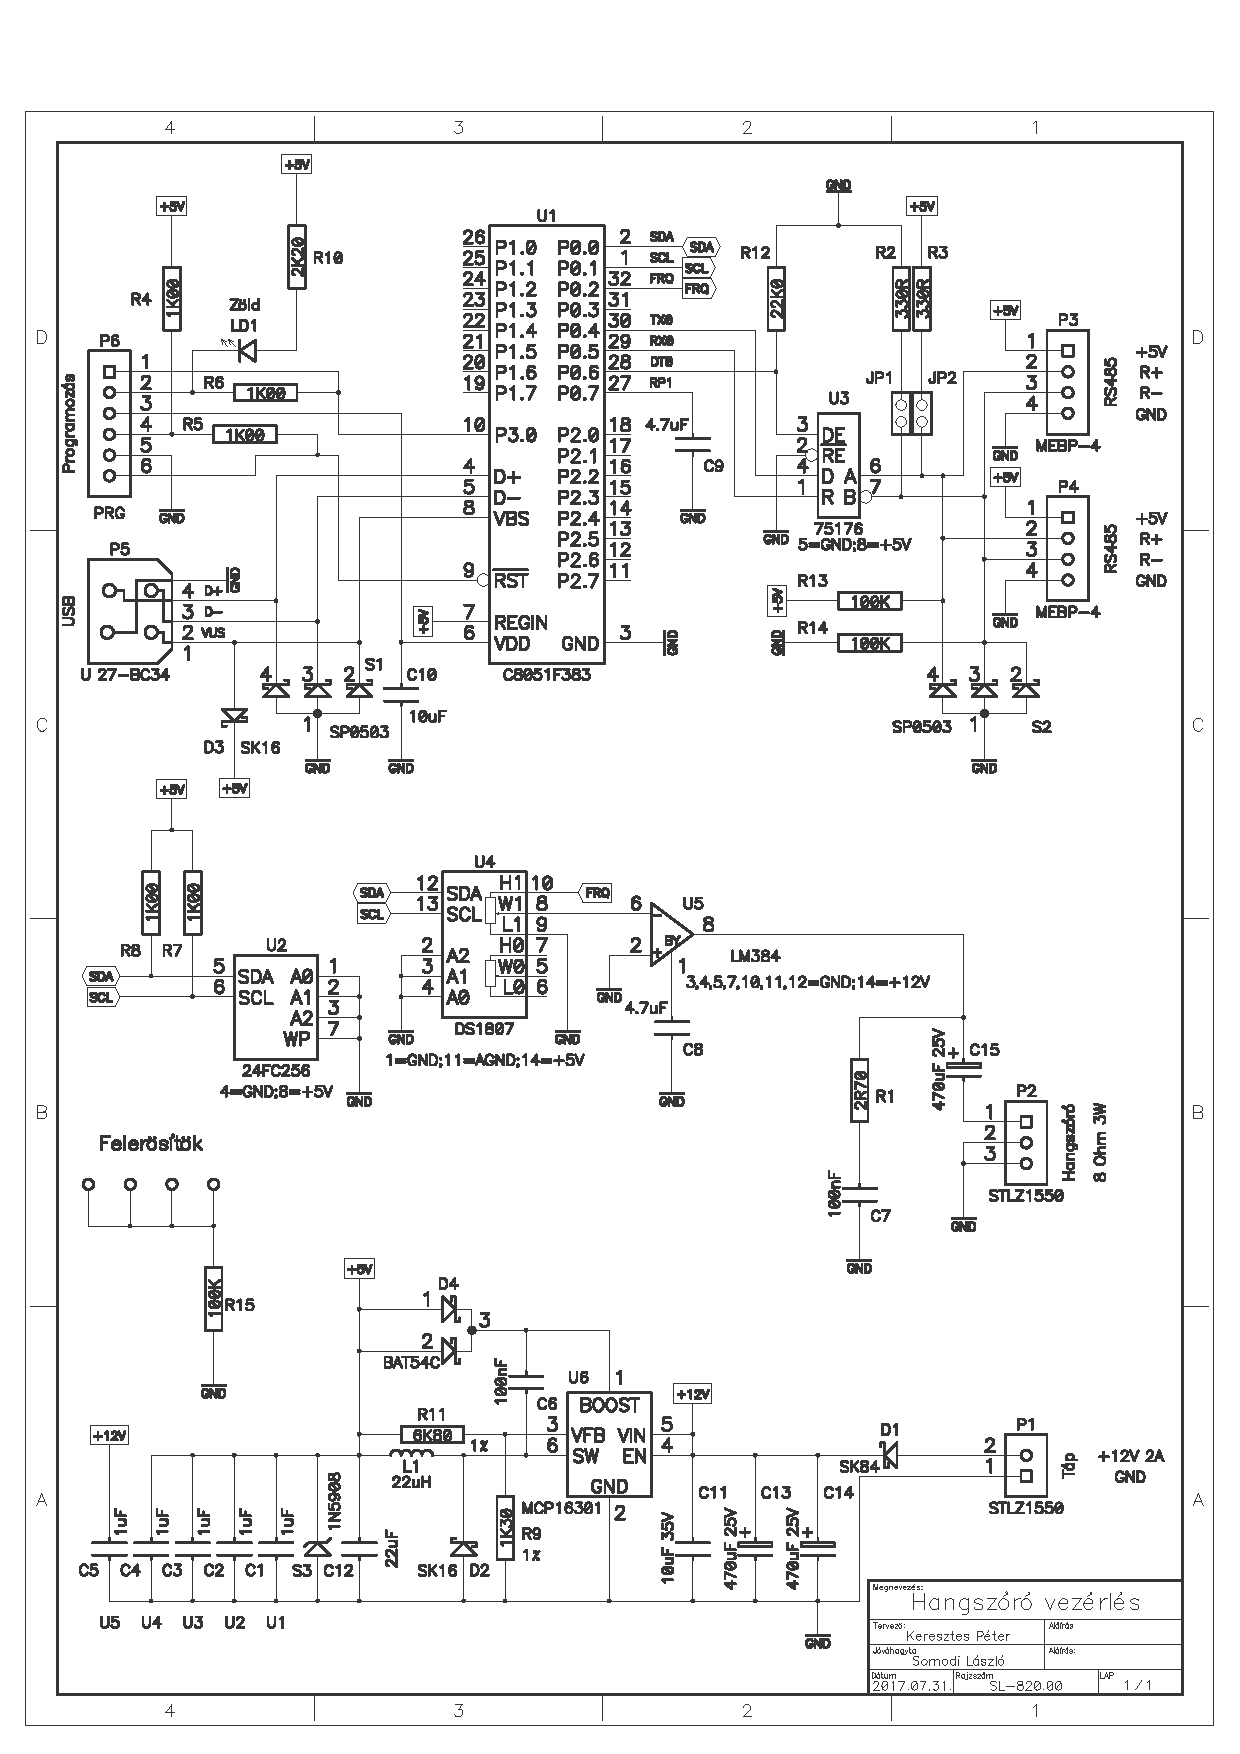
\includegraphics[page=1,width=0.5\textwidth]{SLH}
	\caption[Hangszoró]{hangszóró kapcsolási rajz \#1}
	\label{fig:hangsz1}
	
	\end{figure}
	\begin{figure}[h!]
		\centering
		\includegraphics[page=2,width=0.5\textwidth]{SLH}
		
		\caption[Hangszoró]{hangszóró kapcsolási rajz \#2}
		\label{fig:hangsz2}
	\end{figure}
	\begin{figure}[h!]
	
		\centering
		\includegraphics[page=3,width=0.5\textwidth]{SLH}
		
		\caption[Hangszoró]{hangszóró kapcsolási rajz \#3}
		\label{fig:hangsz3}\medskip
	\end{figure} 


	%lámpa
	\begin{figure}[t]
	
		\centering
		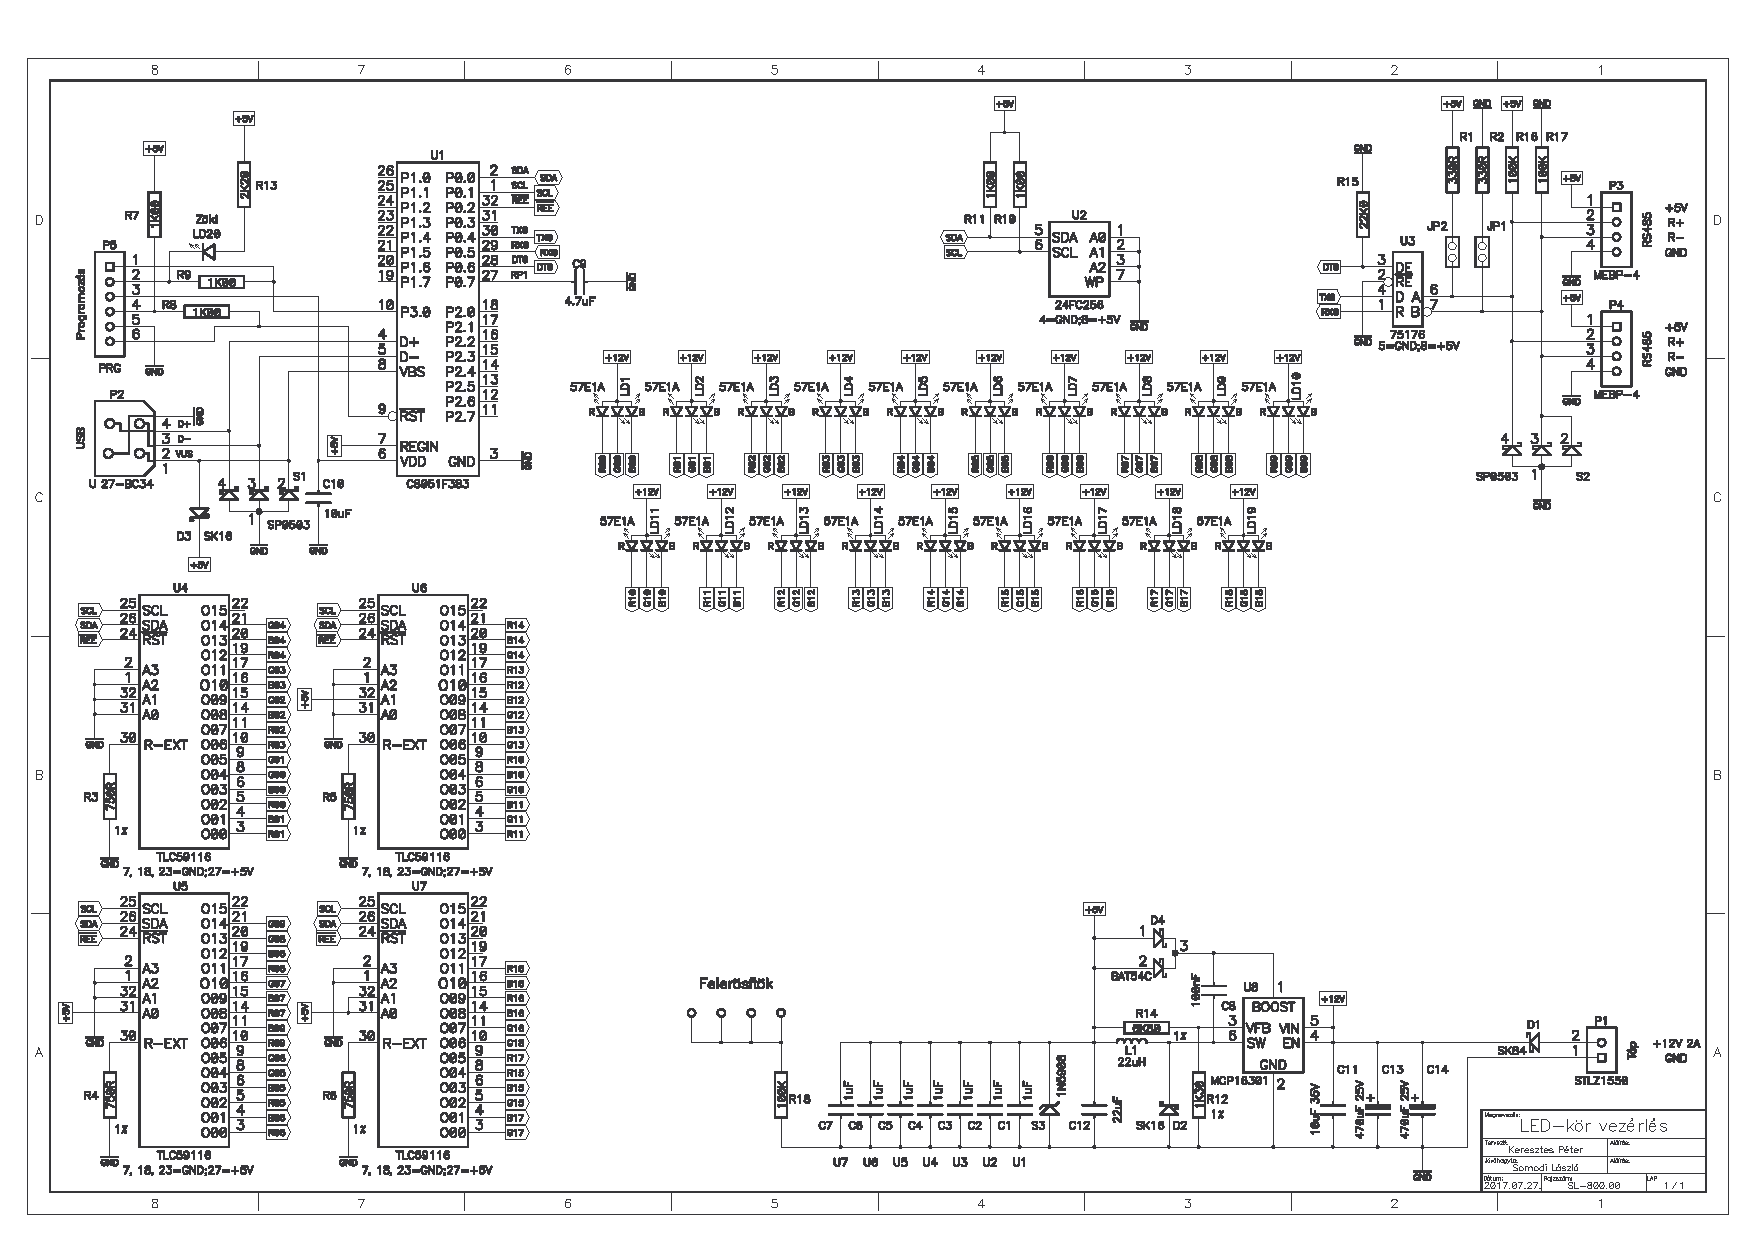
\includegraphics[page=1,width=0.5\textwidth]{SLL}
		
		\caption{lámpa kapcsolási rajz \#1}
			\label{fig:lamp1}
	
	\end{figure}
	\begin{figure}[t]
	
		\centering
		\includegraphics[page=2,width=0.5\textwidth]{SLL}
		
		\caption{lámpa kapcsolási rajz \#2}
		\label{fig:lamp2}
	
	\end{figure}
	\begin{figure}[t]
		
		\centering
		\includegraphics[page=3,width=0.5\textwidth]{SLL}
		
		\caption{lámpa kapcsolási rajz \#3}
		\label{fig:lamp3}
	
	\end{figure}
\par


	%nyíl
	\begin{figure}[h]
		\centering
		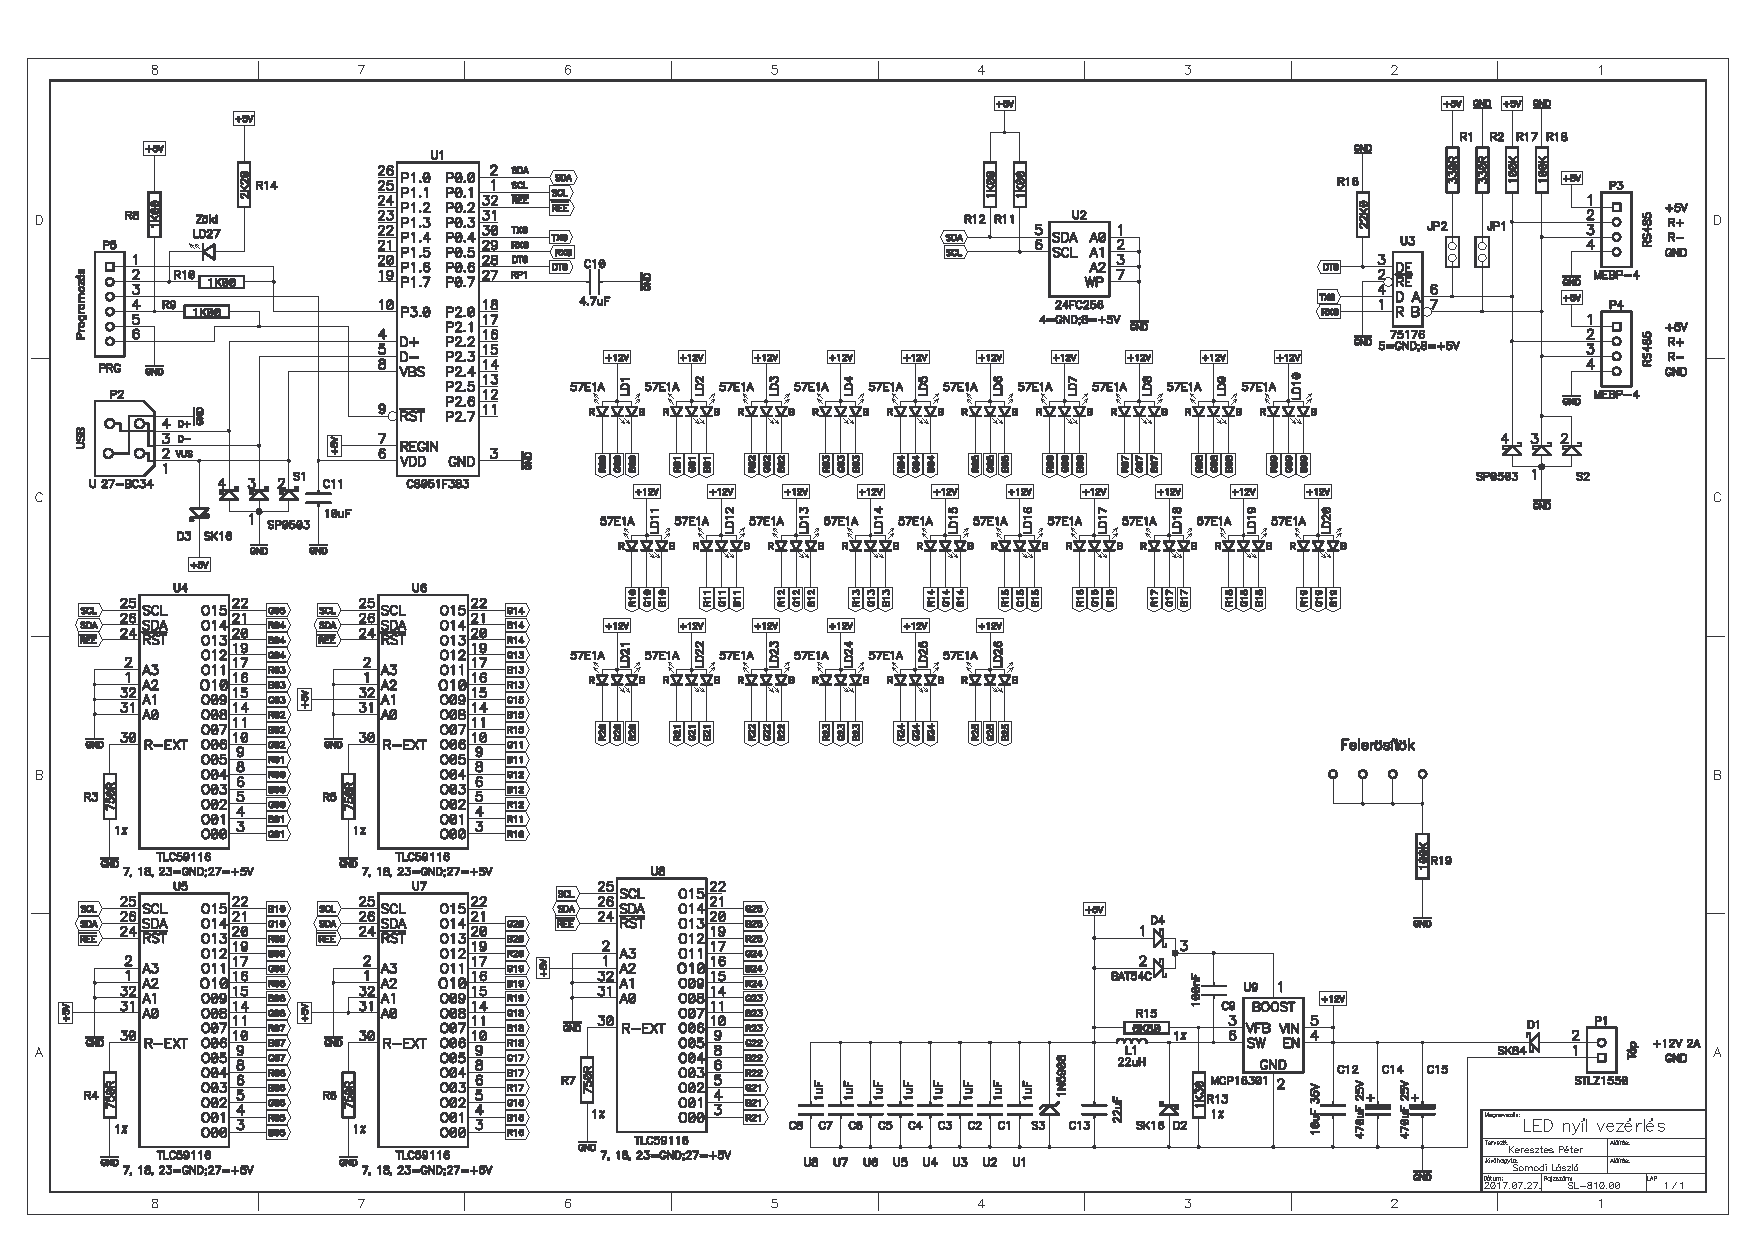
\includegraphics[page=1,width=0.5\textwidth]{SLN}
		
		\caption{nyíl kapcsolási rajz \#1}
		\label{fig:nyil1}
	\end{figure}
	\begin{figure}[h]
		\centering
		\includegraphics[page=2,width=0.5\textwidth]{SLN}
		
		\caption{nyíl kapcsolási rajz \#2}
		\label{fig:nyil2}
	\end{figure}
	\begin{figure}[h]
		\centering
		\includegraphics[page=3,width=0.5\textwidth]{SLN}
		
		\caption{nyíl kapcsolási rajz \#3}
		\label{fig:nyil3}
	\end{figure}




	\begin{comment}
		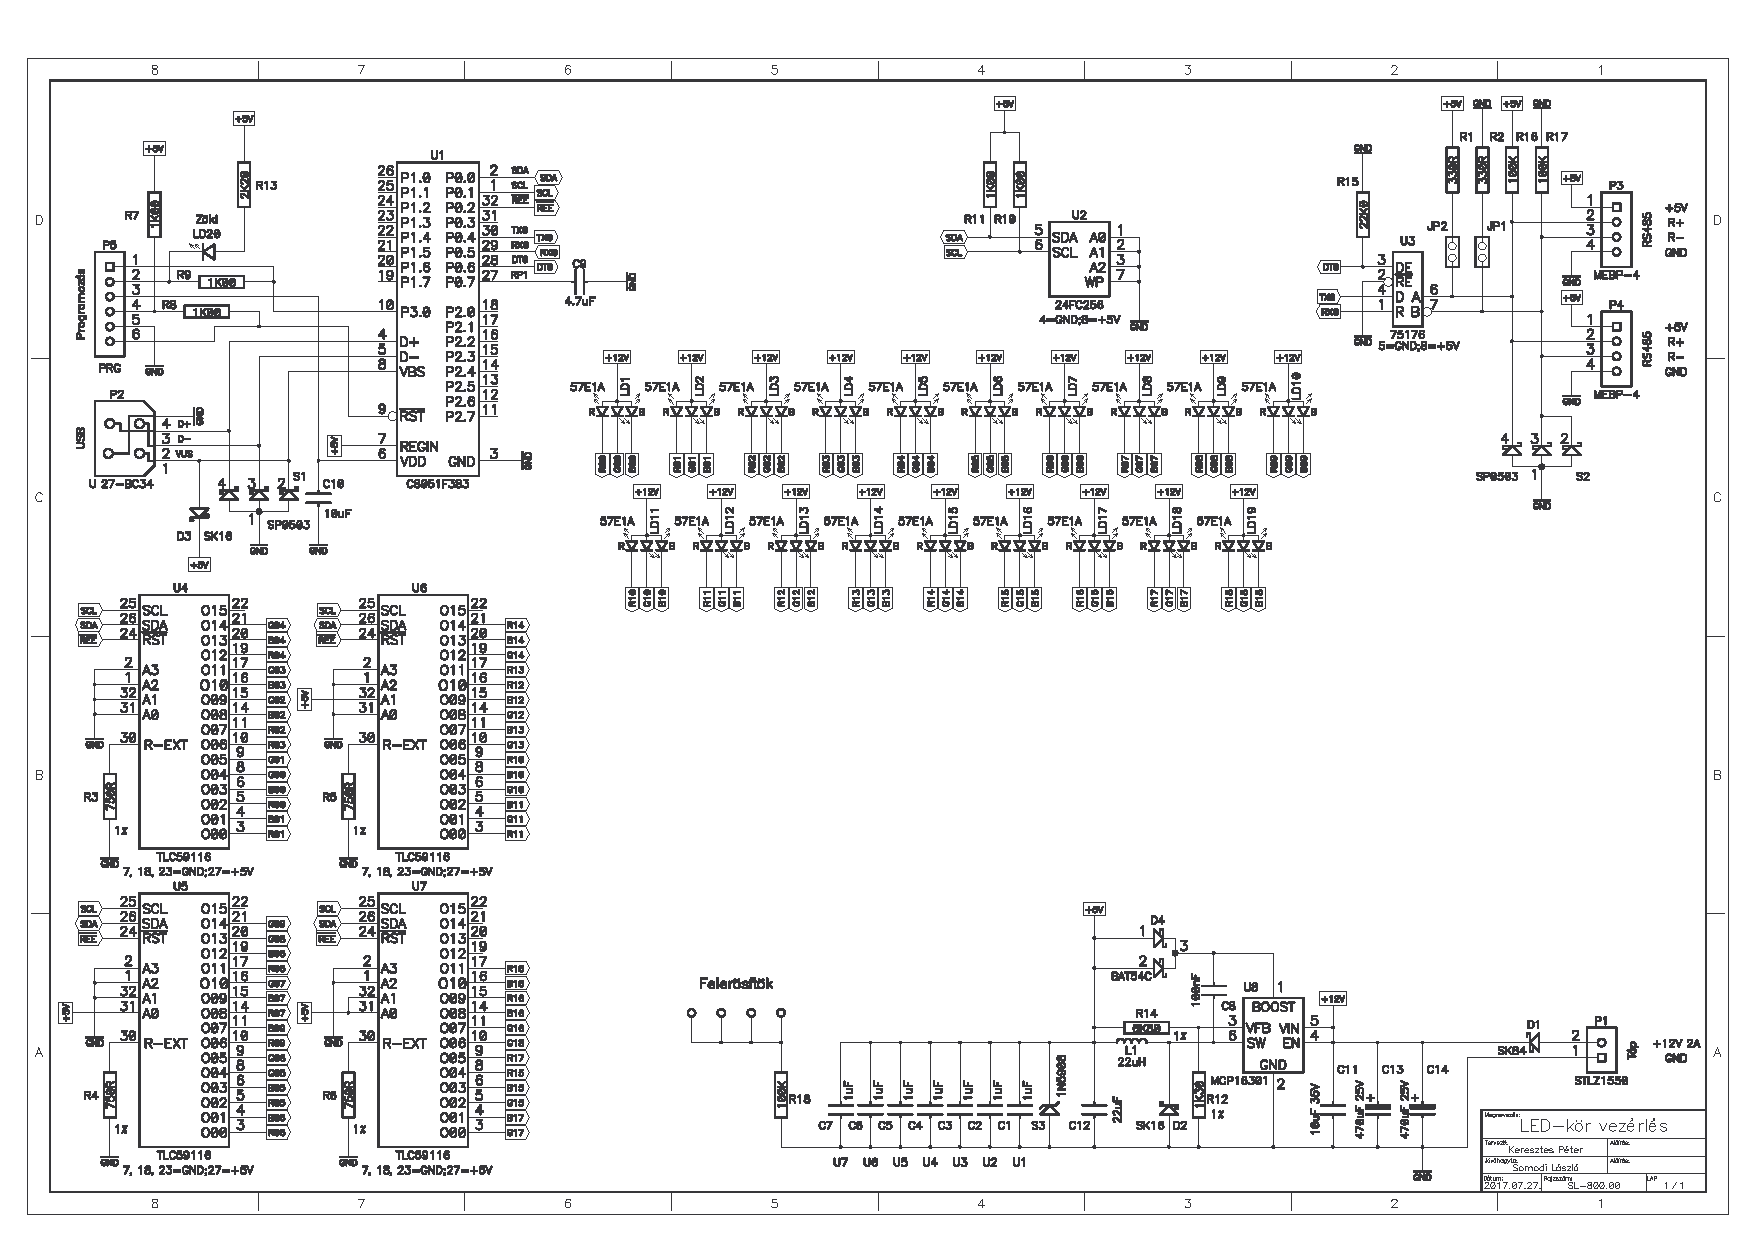
\includegraphics[width=0.5\textwidth]{SLL}
		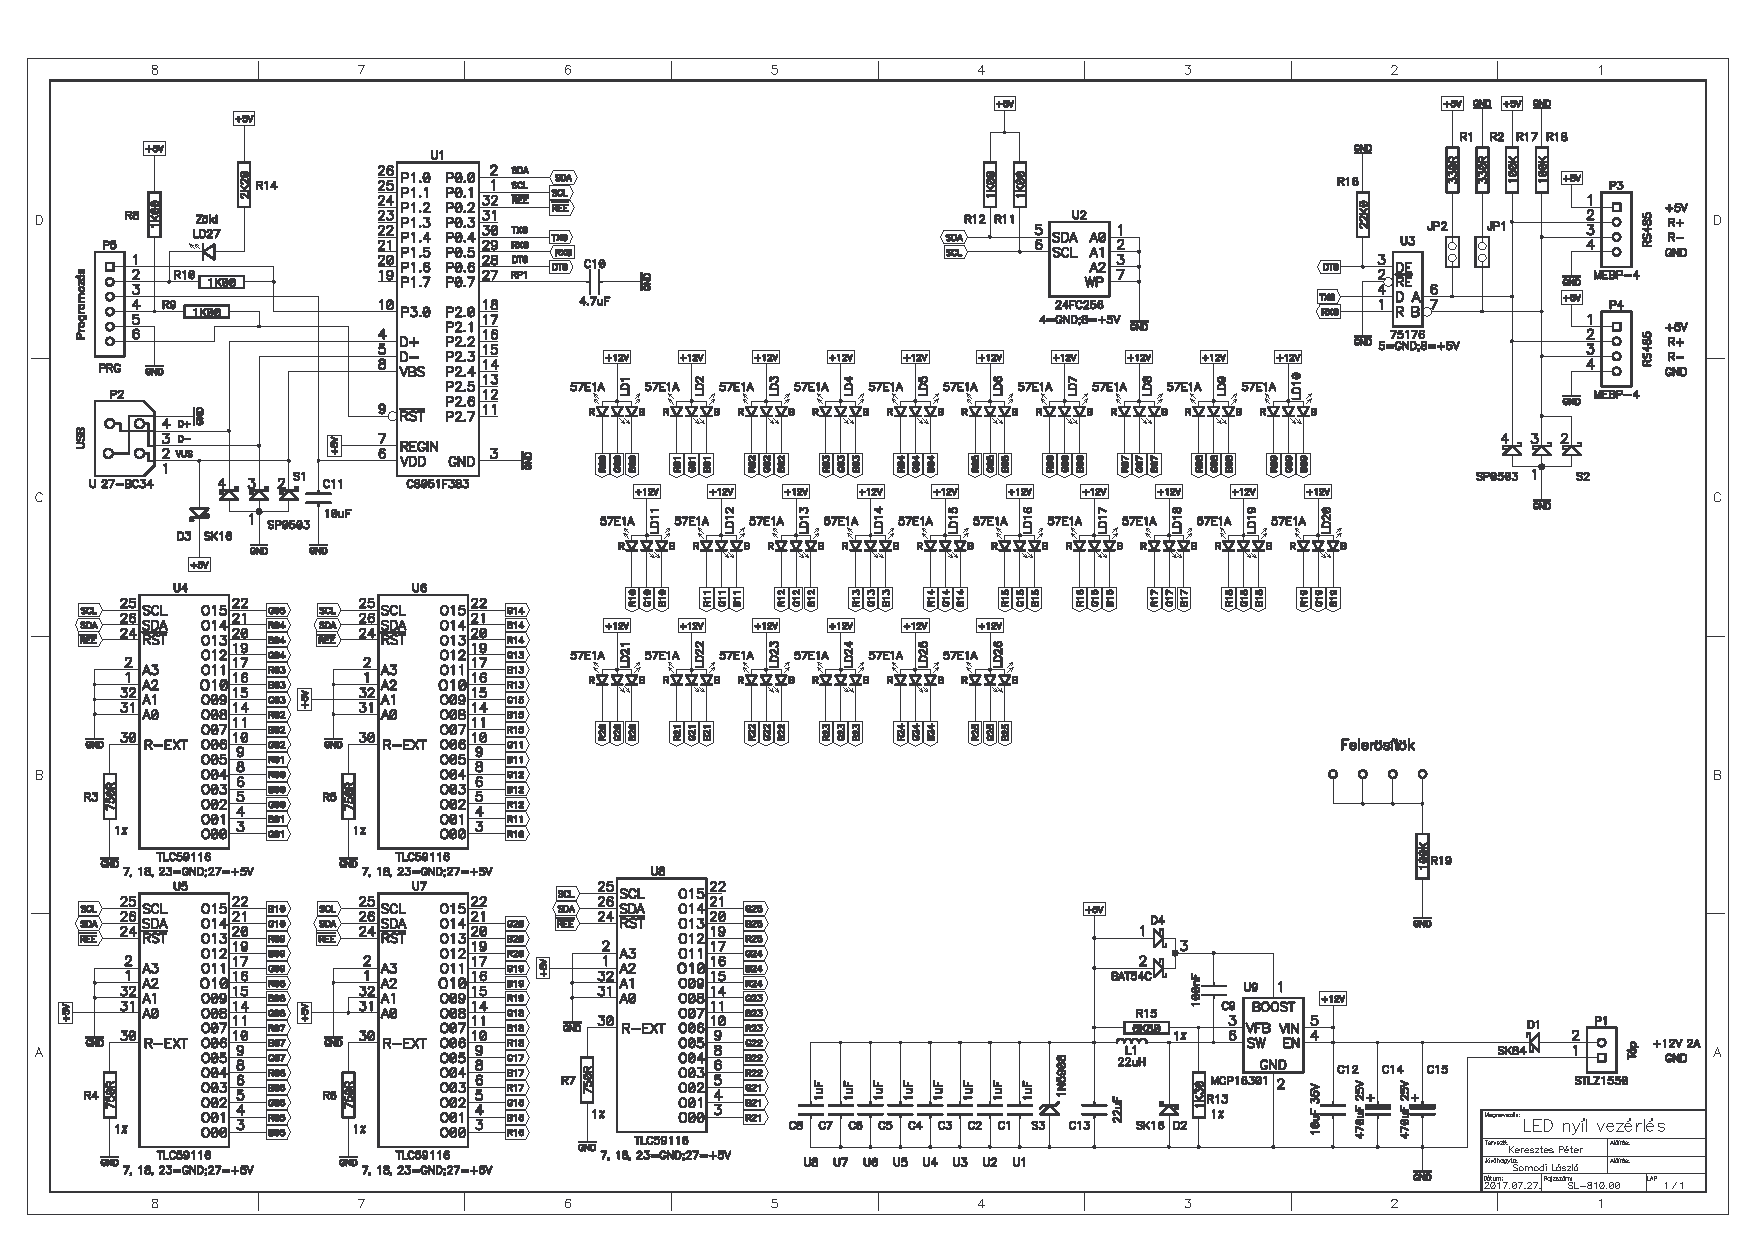
\includegraphics[width=0.5\textwidth]{SLN}
	\end{comment}
	\begin{comment}
		2.fejezet: Melyik részét csinálom én? Mit csináltunk, és hogyan ui-t kellett fejleszteni, milyen lépésekből állt, képernyőképekkel, eladjuk a munkánkat.
	\end{comment}
	\begin{comment}
		2.fejezet: Melyik részét csinálom én? Mit csináltunk, és hogyan ui-t kellett fejleszteni, milyen lépésekből állt, képernyőképekkel.
	\end{comment}
	\chapter*{2.fejezet}
	\section{Felület tervezése}
	A jelenlegi fejezetben magáról a kódról és a felhasználó élményről szeretnék beszélni.
	A korábbi fejezetekben már említést tettem azon kapcsán, hogy az alkalmazást a C\# programozási nyelvben írom. Ezenfelül, egy olyan asztali alkalmazást szerettem volna készíteni amely apelláló lehet a felhasználó számára. Továbbá, a megjelenéstől, és a küllemtől eltekintve fontosnak tartom azt is, hogy egyszerű legyen az alkalmazás használata.
	\\
	Az elkészített szoftver, főleg Windows operációs rendszerrel rendelkező eszközre készül, ez abból is következik, hogy a C\# nyelv kifejezetten a Windows alapú operációs rendszereket támogatja, illetve talán ez a legelterjedtebb operációs rendszer.
	Miután telepítettük a szoftvert azután USB port-on keresztül lehet kommunikálni az adott eszközökkel.
	\\
	%ide még kell az hogy idegen szó a reszponzív szóval bekéne hivatkozni
	A felületnek fontos jellemzője, hogy reszponzív legyen. Amikor a "reszponzív" kifejezést használjuk akkor a "reszponzív kinézetet" értjük. Ez azt jelenti, hogy az adott alkalmazás elérhető és alkalmazkodó legyen mindenféle eszközön. Akár itt értjük azokat az eszközöket amelyeknél nincsen kifejezetten sok beépített periféria, ilyenek például a okos telefonok, tabletek. Az ilyen eszközök során, fontos azt megoldani, hogy az alkalmazásban lévő objektumok(gombok, címkék) könnyen észlelhetőek, és elérhetőek lehessenek a felhasználó számára. 
	Mivel esetlegesen alacsony felbontású képernyőn vagy kis méretű kijelzőn ezek a funkciók nem feltétlen működnének. 
	\\
	Kutatásom során találkoztam egy olyan dizájn formával ami kifejezetten szépnek és modernnek bizonyult számomra.\cite{modernUI} 
	Maga a felület több részből épül fel.
	\\
	\subsection*{Windows Form}
	A Windows Forms-on belül számtalan lehetőségünk van a felületünk megtervezésére. Lehetőségünk van nézetet választani az egyik amely az alap tervezői nézet, és emellett természetesen az alkalmazásunkat kód formájában is megírhatjuk. Számomra a kettő nézet ugyanolyan releváns a projekt szempontjából, mivel a tervezői nézetben, ténylegesen átláthatjuk, hogy a felhasználó mit fog látni mint végtermék.
	
	Amikor a kódnézőben tartózkodunk akkor természetesen eltudjuk érni a ugyanazokat az eszközöket amelyeket a Designer nézetben is.
	Ebben a szekcióban, különböző működési elveket és formai adatokat írhatunk le amelyek meghatároznak különböző objektumokat a form-on belül. 
	\subsubsection*{Designer nézet}
	A nézet választás fontos, és egyben jár a programozás részével is, mivel amikor akár egy gombbot akár egy címkét helyezünk be a képernyőbe akkor is a háttérben történnek változások a kódban is.
	
	A tervezői nézetben egy üres formra építhetünk különböző objektumokat.
	Ez egyszerűbb lehet sok fejlesztő számára mivel, az eszközöket amiket eltudunk helyezni a formunkon mind megtalálható a "Toolbox" nevezetű oldalsávon belül.
	\\
	Itt találunk számos eszközt amelyek bármelyikét használhatjuk a formunkon. Ilyenek például a buttonok vagyis a gombok, vagy a Labelek vagyis a címkék és továbbá elérhetőek még maguk a panelek vagy alpanelek is. Az eszközökről később a  Eszközök [\ref{Eszkozok}] című alfejezetben tárgyalok.
	\\
	Amikor elhelyeztük a kívánt kelléket a formon akkor lehetőségünk van többféle beállításra az adott tárgynál. ezek közé tartozik az az opció amikor egy adott objektumnak a hátterét, címét és még sok más tulajdonságát lehet változtatni a kiválasztott eszköznek. Ezentúl még adott eszköznek lehetnek eseményei is amelyek egy adott impulzus alapján (például: bal klikk lenyomása egy gombbon) kiváltanak egy másik akár látható akár nem látható reakciót a programon belül. Ezekről bővebben az Eszközök című [\ref{EszkozLista}] alfejezetben írok.
	
	\subsubsection*{Alap kód nézet}
	
	A Designer vagy tervezői nézet mellett a programozóknak alkotott nézet is megtalálható a WinForm applikáción belül. Ez a nézet az alap kódolói nézet, amely ugyanolyan fontossággal bír mint a Designer nézet.
	\\
	Amíg a Designer nézetben főleg azon volt a hangsúly hogy a Form-nak vagyis a képernyőnek a nézetét kialakítsuk, megformázzuk. Ezzel ellentétben a kódolói nézetben nem feltétlen látjuk azonnal a kívánt produktumot, mivel ez csak indításkor jelenik meg számunkra, amikor "\textit{lebuildeljük}" a programunkat. Ezt az indítást akár a gyorsbillenytű (\textbf{F5}) segítségével tehetjük meg, vagy a zöld nyílra kattintva a lap tetején.
	\\
	A kódolói nézetben a programozónak lehetősége van minden C\# specifikus elem kihasználására. Alapvetően a minden egyes Gyermek Form örökli a Szülő Form minden public, illetve protected metódusát és mezőjét. 
	\\
	A Formoknál mindig van egy inicializáló konstruktor, amely meghívja a(z) \textit{InitializeComponent()} nevű metódust amely az automatikusan megírt kód alapján előkészíti a form képernyőt a különböző objektumok fogadására. Egyúttal, ez a metódus alapozza meg a gombok, címkék, esemény kezelők és még több ilyesfajta objektumoknak a későbbi beillesztését és használatát.
\\
Ezen kívül, ez a metódus megkeresi a betöltődő Képernyő(Window) és a Felhasználó Vezérlő(UserControl) XAML-jéhez tartozó URI-t.
\\
Majd átadja azt a System.Windows.Application.LoadComponent() nevezetű statikus metódusnak.
Ezt követően, a LoadComponent() nevezetű metódus betölti az átadott URI-n található XAML-fájlt, és átalakítja azt az XAML-fájl gyökéreleme által megadott objektum példányává.
\\
Az \textbf{XAML}(angolul: Extensible Application Markup Language) mint olyan alapvetően egy deklaratív nyelv, amely XML alapján képződött.
Emellett az XAML főleg az olyan típusú eszközök programozásánál használatos amikor felhasználói felületet kell készíteni és programozni. Ilyenek például a Windows Presentation Foundation (WPF) amely sok hasonlósággal rendelkezik a Windows Forms-hoz is.
\\
Az \textbf{URI}(angolul:Uniform Resource Identifier) \cite{uri}
\\
Az \textbf{U} egységesség(Uniform) számos előnnyel jár. Lehetővé teszi a különböző típusú
erőforrás-azonosítók ugyanabban a kontextusban használhatók, még akkor is, ha
az erőforrások eléréséhez használt mechanizmusok különbözhetnek.
\\
Az \textbf{R} olyan a specifikáció amely, nem korlátozza annak körét, hogy mi lehet az erőforrás. Az "erőforrás" kifejezés inkább általános értelemben használatos mindenre, ami URI-val azonosítható. Ilyenek lehetnek az elektronikus anyagok, képek, egy adott információról kapott forrás valamilyen következetes céllal.
\\
Az \textbf{I} az azonosító megtestesíti azokat az információkat, amelyek ahhoz szükségesek, hogy az azonosított dolgot megkülönböztessék az olyan azonosított dolgoktól amelyek az információk hatáskörébe tartoznak.
Az "azonosító" és "azonosítás" arra a célra utal, hogy megkülönböztessenek egy erőforrást az összes többi erőforrástól, attól függetlenül, hogy az milyen célra lett kihelyezve.  
	\subsection{Eszköztár}
	\label{EszkozLista}
	Az eszközök listáját használhatjuk a Designer nézetben. Ezzel a módszerrel, könnyedén tudjuk mozgatni az adott eszközöket. Emellett, az Eszköztár ablakban a vezérlőelemek jelennek meg.Az eszköztár megnyitásához a menüsorból a Nézet > Eszköztár parancsot kell megkeresni, vagy a \textbf{Ctrl+Alt+X} billentyűzetkombinációt kell megnyomni. Ilyenek például a gomb, címke, panel. Az eszköztár a tervezői nézetekkel együtt jelenik meg általában. 
	\\
	Az eszköztárban lehetőségünk nyílik szűrni is különféle eszközökre, ezt megtalálhatjuk a \textit{Search Toolbox} nevezetű kereső mezőben.
	\subsubsection{Gombok}
	\label{Gombok}
	A gombok általánosságban olyan fontos elemei a felületnek és a Formnak is amelyeken keresztül nem csak a programozó kommunikálhat a felhasználó felé, de a felhasználó is kommunikálhat a program illetve a programozó felé. 
	\\
	Ezentúl még a gombok hasznosnak bizonyulnak sok különböző helyzetben is mivel a gomboknak és más objektumoknak is, léteznek úgynevezett eseményei. Ezen eseményeket (Angolul: "Event") a felhasználó ki tudja váltani különböző cselekedetekkel. Ilyen esemény lehet példaként az amikor a felhasználó a bal egér gombbal kattint a gomb felületére, ezzel kiváltva egy eseményt ami bekövetkezik ezen okból kifolyólag.
	\\
	Tervezői nézetből egy gomb esemény kialakítása többféle módon történhet. Amikor kihelyezzük a használni kívánt gombot akkor lehetőségünk van, vagy a jobb alsó sarokban megjelenő "\textit{Properties}" nevezetű ablakon belül navigálni vagy egyszerű módon csak kétszer kattintunk a létrehozott gombra, ezzel a programunk legenerál számunkra egy "xyz\_Click()" metódust.
	Az elsőnek említett módban, a "\textit{Properties}" nevezetű ablakon belül, az apró villám ikonra kell kattintanunk, amely az adott objektumhoz tartozó események listáját tárja szemünk elé. Ez megkönnyítheti a kereséseinket, hogy éppen az adott objektumra milyen események lehetségesek. További információt majd a \ref{esemenyformban} fejezetben fejtenék ki.
	\subsubsection{Címkék}
	\label{Címkék}
	A címkék általánosságban megtalálhatóak minden programban felületén. Ilyenek például az üdvözlő üzenetek, címek, szöveges magyarázatok.
	%ide akár lehetne ezekről ilyen képeket is betenni a címkékről
	A címkék alapvetően nem arra szolgálnak, hogy a felhasználó tudjon kommunikálni a programozóval/programmal, hanem arra, hogy a fejlesztő tudja továbbítani a programozó által írt szöveges üzeneteket a felhasználó számára. Hasznos lehet olyankor amikor a felhasználóval tudatni akarunk olyan információkat amelyek a  program működéséhez releváns volna. Ennek egy példája amikor egy adott gombnak a funkcióit szeretnénk leírni, ilyenkor a címke arra szolgál, hogy feliratozzuk az adott funkciókat a programunkon belül.
	\\
	  Természetesen mind a kétféle nézetben(designer/kód) elérhető számunkra a címkék használata, de meg kell fontolnunk, hogy kód nézetben alapvetően nem látjuk azonnal azt amit a felhasználó is látni fog, ezért talán nehézségekbe ütközhetünk ilyenkor ha manuális szeretnénk kód formájában megadni a címke paramétereit, beállításait. Amennyiben designer nézetben helyezzük el a címkénket könnyebben és rugalmasabban tudunk a programunkkal dolgozni, de sajnos ennek is megvannak a hátrányai, ha a program futási idejében szeretnénk változtatni akkor használnunk kell a kód nézetet is amellyel kiegészítve megtudjuk oldani ezeket a felmerülő problémákat is. Ebből kifolyólag hasznos lehet a designer nézet és a kód nézet együttes dinamikus használata.
	  \\
	  Mivel a címkék is szövegek/stringek ezért egy adott címkének el lehet érni a szöveg formátumát sok más beállításával együtt. Ilyenkor ha stringet szeretnénk esetlegesen konkatenálni, abban az esetben az adott label-nek a \textit{Text} nevezetű property-jét kell lekérdeznünk. Majd ezt követően használhatjuk a címkénk szöveg adására, illetve kiegészítésére.
	\\
	Későbbiek során természetesen ez a funkció is szerves részét alakítja az elkészült programnak.
	\subsubsection{Panel}
	\label{Panel}
	A formnak mint olyannak léteznek paneljei. Ezen panelek hasznosnak bizonyulnak sok szempontból. Legfőképpen a háttér díszítéséhez, objektumok összegzésére lehet használatos. Jelen alkalmazásban is két fő részében használom a projektnek. 
	Oldalsávhoz használtam fel a panelt, illetve a fejléchez. 
	\\
	Ahhoz, hogy a panel fejléc illetve oldalsávként funkcionáljunk néhány beállítást kellett elvégezni a panelen. A fejléc kialakítását az úgynevezett \textbf{Dock} nevezetű beállítással lehet konfigurálni. 
	 \\
	 A Dock abban segít hogy egy adott objektumot a képernyő egy adott részére helyezze, feltűzze. A megoldás segít abban, hogy reszponzív maradjon a felület, és egy szép kialakítást biztosít számunkra a megjelenítést illetően.
	 \\
	 Az oldalsávot is hasonlóképpen lehet megoldani, mindösszesen a Dock beállítást kell bal vagy éppen jobb oldalira konfigurálni, és ezzel a képernyő oldalához illeszti a panelt.
	\subsection{Delegatek}
	\label{Delegateek}
	A delegatek a C\# nyelven belül, mindig egy hivatkozás. Egy olyan hivatkozás amely mutat egy metódusra. Amennyiben egy delegatet hívunk akkor a hivatkozott metódus lesz meghívva. A delegateknek megvan minden szükséges információjuk ahhoz, hogy hívják egy adott egyedi névvel és visszatérési típussal ellátott metódust vagy metódusokat.
	\\
	A delegateket átadhatjuk egy másik metódusnak is ezzel áthelyezve a metódusnak a felelősséget a híváshoz, vagy éppenséggel egy struktúrában vagy osztályban is tárolhatjuk a delegatejeinket. A delegateket akkor használjuk, amikor nem tudjuk, hogy melyik metódust fogjuk meghívni tervezés közben, hanem csak futás közben derül ki ez.
	\\
	A delegatek deklarálásához szükséges a \textbf{delegate} kulcsszó amelyet követően meg kell adni a visszatérési értéket és a delegate nevét és paraméterét.
	\\ 
	Ezt követően meg kell írnunk a hivatkozni kívánt metódust, majd ezek után a delegatet és a metódust összekötjük úgy, hogy a delegatet lepéldányosítjuk és a new kulcsszót és a delegate nevét követően paraméterben megadjuk a kívánt metódust. 
	\\
	A delegatekre a későbbiek során csak az eventek során lesz szükségünk, mivel az eventek alapját képzik a delegate-k
	\subsection{Események}
	\label{Eventek}
	Az események vagy eventek \cite{evinC} a C\# nyelven belül, olyan mechanizmusok, amelyeket az osztályok használnak értesítések vagy üzenetek küldésére más osztályoknak. Az események számos alkalmazás létfontosságú részét képezik, és tökéletes módja annak, hogy rugalmas és bővíthető alkalmazásokat hozzunk létre.
	Az elkészített alkalmazás is számos helyen alkalmaz, eventeket amelyek általában gombok lenyomásakor történnek meg.
	\\
	\subsubsection{Esemény készítése}
	Ahhoz hogy egy eseményt megalakítsunk szükség van egy kiadóra, aki az eseményt létrehozza, majd az esemény fogadásához és kezeléséhez elengedhetetlen egy fogadó is aki feliratkozik az esemény fogadására.
	
	\subsubsection{Esemény a gyakorlatban}
	Az event emellett általában a megfigyelő tervezési mintával kapcsolatban használják. Amikor ugyanis egy ilyen esemény bekövetkezik a feliratkozott figyelők csoportja meg lesz szólítva és ezzel kapnak információt a bekövetkezett eseményről. Azok az objektumok amelyek "érdekeltek" abban, hogy fogadjanak értesítéseket az eseményről, azok regisztrálnak egy delegate példányra az eseményhez.
	Egy esemény mindig a vele együtt elérhető delegattel van definiálva. 
	Az eseményt mindig egy delegattel kell együtt használni.
	\\
	Egy esemény értéke \textbf{null}, ha nincs regisztrált/feliratkoztatott figyelője/hallgatója.
	\subsubsection{Esemény működtetése a formban}
	\label{esemenyformban}
	Egy Formban általában alap eszközökre vagy objektumokra hozhatunk létre eseményeket, ilyenek például egy gombra való kattintás, vagy esetlegesen egy textbox nevezetű elem amelybe éppen megváltoztattuk a szöveg tartalmát.
	Számos lehetőségünk van az ilyen eszközökből kiváltani eseményeket.
	Az események létrehozásáról már a \ref{Gombok} számú fejezetben említést tettem.
	Miután elkészítettük ezeket az eseményeket akár a "Properties" ablakban akár másféle módon utána a létrehozott metódusunk egy \textbf{private} láthatósági móddal rendelkező metódus lesz, amelynek visszatérési értéke \textbf{void} vagyis visszatérési értékkel nem rendelkezik. 
	\\
	Ezentúl, paramétereiben kettő objektumot kap meg a metódus, egyrészt egy \textbf{object sender} amely az eseményt kiváltó vezérlőre/objektumra való hivatkozást tartalmazza. Tegyük fel, hogy egy képernyőn több gomb van. Ezek a gombok tartalmazhatnak egy címkét, amely leírja, hogy mit kell tennie a gombra kattintva. Ezáltal az összes \textbf{"Click"} eseményt lehetséges lekezelni ugyanazzal a handlerrel.
	Emellett egy \textbf{EventArgs e} objektumot amely az eseményadatokat tartalmazó osztályok alaposztályát képviseli, és egy olyan értéket biztosít, amelyet az eseményadatokat nem tartalmazó eseményekhez kell használni. 
	\cite{eventobjargs}
	
	\subsection{A Formról általánosan}
	A képernyőket próbáltam megoldani az előzőekben említett módon, hogy reszponzív lehessen vagyis mindenféle képernyőn hasonlóan jól és szépen megjelenhessen. Ehhez kutatásom során találtam egy megoldást amely szerint, ha az adott Form-nak a méretét(Size) beállítom az elsődleges képernyőnek a méretére, illetve a képernyő állapot nevű változót is egyenlővé teszem a "FormWindowState" enumból a Maximized értékére akkor a képernyő ideális, kinagyított állapotba kerül. A módszer, megoldást nyújthat arra, hogy a képernyőn teljes méretbe jelenjen meg minden egyes objektum amit az adott képernyőre helyeztünk. Ezen beállításokat az adott Formnak a konstruktorában hívjuk meg.
	\\
	A címke kiíratását úgy tudtam megoldani, hogy az adott Form-on belül a Toolbox nevezetű eszközt használva, kiválasztottam a "Label" ikont amely segítségével szövegeket/stringeket tudunk kiíratni. Természetesen ezt akár a kódon belül, Design nézet nélkül is meglehet oldani, de jelen helyzetben a Design nézetféle megoldást tartottam hasznosabbnak. Ezt követően a kódon belül ennek a címkének, a Text változójához hozzáadtam a kívánt szöveget, meg az eszközök darabszámát is, mint változót.



	\subsection{SzinTema osztály}
	A \textbf{SzinTema} nevezetű osztály egy külön készített nem beépített osztály, amely a színváltozásokat és az alap színkódokat tárolja el.
	A színkódokat egy Listában tároljuk el amelyből majd a későbbiekben a Form Main Menu Form választja ki a megfelelő színeket. Ehhez a listához van egy \textbf{getColorList()} metódusa is amely a listának az elérésére szolgál. 
	\\
	A másik metódus az a \textbf{ChangeColorBrightness()} metódus amely paraméterében vár egy \textbf{Color} példányt illetve egy korrekció faktort amely a színek korrigálását fogja végezni, ezzel elérve a várt színárnyalatokat. Amennyiben túl sötét lenne a szín vagyis a korrekció faktor nagyobb lenne mint 0 akkor a színét kivilágosítjuk, ellenkező esetben a korrekciófaktort növeljük 1-el és megszorozzuk őket a piros, zöld, illetve a kék színértékekkel. Ezt követően visszatérési értékként visszaadjuk a megkapott színt mint visszatérési érték. 
	\subsection*{Form Main Menu}
	\label{FormMainmenu}
	Az első Form, a főmenü, vagyis amikor a felhasználó megnyitja az alkalmazást akkor ez az első képernyő ami számára megjelenik. 
	Ezen képernyőn egy üdvözlő üzenetet kap, majd az észlelt eszközök darabszámát is látni fogja, amely ugyanúgy megjelenik a képernyőn.
	Az üdvözlő üzenet, a fejlécen, a Form tetején jelenítjük meg amely egy Panel segítségével kapott színes hátteret.
	\subsubsection{Konstruktor}
	A kezdő menünek a konstruktora sok adatot tartalmaz a formmal kapcsolatban. Alapvetően az első és legfontosabb elem az a \textit{InitializeComponent()} metódus amely az automatikusan megírt kód alapján előkészíti a form képernyőt a különböző objektumok fogadására.
	\\
	 A kinézethez nagyban hozzájárult a(z) \textbf{EnableVisualStyles()} nevezetű metódus amely a(z) \textbf{Application} osztály egy metódusa. Az említett metódus akár félreérthető lehet, mivel első gondolatra lehetséges, hogy a fejlesztő arra asszociál, hogy a metódus segíti a Form-ban lévő objektumokat, vizuálisan kirajzolni. Valójában amikor ez a metódus fut, akkor a beépített Windows rendszer témájától függően alakítja az említett gombokat, címkéket, és további objektumokat. Amennyiben a használt gép beépített stílusok nélkül fut abban az esetben a felhasználó nem fog semmilyen változást észlelni a program/felület használatakor.
	\subsubsection{SelectThemeColor metódus}
	A \textbf{SelectThemeColor()} metódus egy adott oldal fejlécének a színét fogja beállítani. A következő sorokban ezt taglalnám, miként és hogyan teszi ezt. 
	\\
	Elsőnek beállítunk egy index nevezetű változót ami egy véletlenszerűen választott értéket választ a \textbf{SzinTema} nevezetű osztály \textbf{ColorList} listájából. A véletlenszerű kiválasztást a \textbf{Random} osztály \textbf{Next} metódusával érjük el, amely a jelenlegi helyzetben egy 0-tól a \textbf{lista.Count}-ig megy ami a listának a teljes hosszát tartalmazza, vagyis azt, hogy a listában mennyi elem szerepel. 
	\\
	Ezt követően megvizsgáljuk a metóduson kívül létrehozott \textbf{tempIndex} nevezetű értékünket és a most megkapott \textbf{index} nevezetű változónkat, és ameddig a két érték megegyezik egymással addig léptetünk az \textbf{index} változón. Ez a ciklus ez azért szükséges, mivel ha nem létezne ez a lépés akkor első belépésünk után ugyanazokat a színeket kapnánk mindegyik képernyő esetén. 
	\\
	Majd a \textbf{tempIndex} változónkba eltároljuk az \textbf{index} nevezetű változónk értékét, majd ezután a visszatéréshez szükséges \textbf{color} változónkba eltároljuk az \textbf{index} helyen található, szín kódját. Majd az így kapott értékkel térünk vissza, melyet a(z) \textbf{ColorTranslator} osztály \textbf{FromHtml()} nevezetű metódusán keresztül fordítunk át tényleges \textbf{ARGB} színként.
	
	
	\subsubsection{ActivateButton metódus}
	A(z) \textbf{ActivateButton()} paraméterében vár egy \textbf{btnSender} nevezetű objekt típusú változót, emellett visszatérési értéke a metódusnak nincsen. A \textbf{btnSender} változót megvizsgáljuk hogy a benne lévő érték üres-e vagyis \textbf{null} értékkel egyenlő-e vagy sem. Amennyiben van a változóban érték, ekkor megvizsgáljuk hogy a metóduson kívül létrehozott \textbf{currentButton} változónkkal megegyezik-e a paraméterben kapott változó. Amennyiben a két érték nem egyezik akkor meghívjuk a \textbf{DisableButton()} nevezetű metódusunkat amelynek a kifejtését a \ref{Disablebuttonlabel} számú alfejezetben írom le.
	\\
	 Majd ezután egy átmeneti \textbf{color} változóba elmentjük a \textbf{SelectThemeColor()} metódusból származó szín értékét. Ezt követően a \textbf{currentButton} változót beállítjuk a paraméterben kapott változójaként, majd ennek a \textbf{currentButton} változó beállításait konfiguráljuk. Ezt követően a fejléc színét is beállítjuk a kapott \textbf{color} változóra, és a \textbf{SzinTema} nevezetű osztály elsődleges (angolul: primary) változóját beállítjuk a \textbf{color} változóra majd ahhoz illesztve a másodlagos (angolul: secondary) szín értékét beállítjuk a \textbf{ChangeColorBrightness()} nevezetű metódusnak az értékére, melyet a \textbf{color} változó és a korrekció faktor alapján számít ki.
	 \\
	 Végül a gombot amely az alaphelyzetbe állítását végzi a formnak, azt a gombot igazra (angolul:True) állítjuk.
	\subsubsection{DisableButton metódus}
	\label{Disablebuttonlabel}
	A \textbf{DisableButton} metódus azért képezi fontos részét az alkalmazásnak mert amikor a felhasználó navigál a gombok között akkor kattintásával megváltoztatja az adott gombnak a háttérszínét is. Ez a funkció színesebbé teszi a formot és felhasználó barátibb lesz a rendszer maga. Ebben a metódusban ezt a színváltoztatást úgy érhetjük el, hogy a \textbf{panelMenu}-nek a \textbf{Controls} mezőjét végigjárjuk egy ciklussal és megvizsgáljuk, hogy az adott \textbf{Control} típusú változónak a típusa az gomb-e.
	Amennyiben a bool értéke a feltételnél Igaz abban az esetben az adott gombnak a háttérszínét és szövegtípusát megváltoztatjuk.
	\\
	Ellenkező esetben ha a feltétel kiértékelésénél Hamis értéket kapunk akkor nem változtatjuk meg az adott \textbf{Control} típusú változó értékeit.
	\\ 
	Ez a feltétel kiértékelés azért fontos mivel ha nem vizsgálnánk meg azt hogy az adott \textbf{Control} típusú objektum gomb-e, akkor az összes gombnak a színezése változatlan állapotba maradna.
	\subsubsection{OpenChildForm metódus}
	Az \textbf{OpenChildForm()} metódust arra fogjuk használni, hogy előző formban lévő adatokat, színeket átadjuk a másik következő formnak. Amikor rákattint a felhasználó az adott gombra, akkor ezt az eljárást hívjuk meg melynek paramétereiben megadjuk a kívánt formnak az objektumát, és a \textbf{sender}-t amely a gombnyomás metódus paraméteréből származik. A jelenlegi eljárásban, az éppen aktív formnak értékül adjuk a kattintáskor megadott form értékét. Ezt követően a paraméterben kapott form beállításait változtatjuk, majd megjelenítjük ezen formot. 
	\subsubsection{Reset metódus}
	A \textbf{Reset} metódus meghívja a \textbf{DisableButton()} nevezetű metódust mely alaphelyzetbe állítja az oldalsávban lévő gombok színét, és stringjük méretét.
	\\
	Ezt követően a címhez tartozó címke \textbf{Text} változóját átírjuk \textbf{HOME}-ra, és mindent alapbeállításokra állítunk. Ezek tartalmazzák a címke átírása mellett a háttérszín alapszínre állítását, illetve a gyermek formot bezáró gomb láthatóságának false-ra vagyis hamisra állítását is.
	\\
	\subsubsection{Oldalsáv}
	Az alap formunk még egy oldalsávból is áll a kezdőképernyőnk amely navigációt és könnyebb tájékozódást jelenthet a felhasználó számára.
	Ebben a sávban gombok helyezkednek el amelyeknek, külön hátterük, és ikonjuk van. Ezek mind hozzájárulhatnak a felhasználó-barát szemléletmódhoz.
	\\
	A navigáció sávban megtalálhatjuk a következő gombokat:
	\begin{itemize}
		\item Indítás
		\item Feladatsor Mentés
		\item Feladatsor Betöltés
		\item Feladatsor Szerkesztés
		\item Kilépés
	\end{itemize}
	Az indítás gomb...
	%még nem tom mi kéne ide
	\\
	A Feladatsor Mentés gomb...
	Ennek a gombnak a segítségével a jelenlegi eszközöknek a beállításait mentheti el a felhasználó, amennyiben számára az eszközök elérhetőek. A funkció kifejtését és a megoldását a későbbiekben, a Form Mentés \ref{Form Mentes} alfejezetben fejteném ki.
	\\
	A Feladatsor Betöltés gomb...
	A gomb használatával a felhasználó képes betölteni adott eszközökhöz tárolt adatokat, mint például: adott lámpákhoz tartozó LED-ek színét, vagy adott nyilakat ábrázoló eszközöknek a színét illetve irányát, vagy esetlegesen a hangszínt, hangerősséget, és még a hanghosszt adott hangszórók esetén.
	Ezeknek kifejtését a Form Betöltés című \ref{Form Betoltes}
	alfejezetben fejtem ki.
	\\
	A Feladatsor Szerkesztés gomb...
	Ezen gomb használatával a felhasználó tudja szerkeszteni a már ismert eszközöket. Akár az adott lámpákhoz tartozó LED-ek színét, vagy adott nyilakat ábrázoló eszközöknek a színét, illetve azok irányát, vagy esetlegesen a hangszínt, hangerősséget, és még a hanghosszt adott hangszórók esetén.
	Ezeknek a kifejtését a Form Szerkesztés című \ref{Form Szerkesztes}	alfejezetben fejtem ki.
	\\
	A Kilépés gombot arra használhatja a felhasználó, hogy az alkalmazást terminálni tudja. Ez a problémát egy gomb segítségével oldottam meg. A gombnak van egy olyan eseménye, hogy "MouseDown" amely segítségével egy olyan eseményt tudunk kiváltani amely akkor történik meg amikor a felhasználó lenyomja a gombot a bal egérgomb segítségével.
	Ehhez az "event"-hez kötöttem egy Exit() metódust ami az Application osztáynak az egyik metódusa. Ez a metódus bezárja az applikációt, és befejezi a program futását. 

	\subsection{Form Mentés}
	\label{Form Mentes}
	A \textbf{Form Main Menu}-n kívül az összes másik formot az \textbf{OpenChildForm()} metódussal hívunk, így a feladatsor mentésre is kialakított formot is ezzel a metódussal hívjuk. Alapvetően, a mentés form arra lesz hivatott, hogy azokat az eszközöket amelyek érzékelve vannak a rendszer által kimentse, egy JSON file-ba.
	\\
	A JSON azért optimális fájl formátum mivel közismert és tökéletes arra, hogy átmeneti adatot tároljunk benne. 
	\\
	Ilyen átmeneti adat lehet egy felhasználó által generált adat, vagy például a jelenlegi helyzetben az eszközök beállításai. 
	\\
	A mentést a \textbf{Feladatsor Mentése} gomb megnyomásával válthatja ki a felhasználó. Ezt követően pedig ki kell választania a felhasználónak, hogy hova szeretné elmenteni a \textbf{JSON} fájlban eltárolt eszközök adatait.
	\\
	A mentés azért is lehet optimális funkció mert ha a későbbiekben szükségünk volna egy adott beállításra, akkor lementjük az eszközök adatait és amikor újra szükségünk lesz betöltjük azokat a \textbf{Feladatsorok Betöltése} gombbal. Későbbiekben a betöltésről a \ref{Form Betoltes}
	\subsubsection{Konstruktor}
	A mentés formnak a konstruktora hasonlóképpen épül fel mint a \ref{FormMainmenu} fejezetben lévő konstruktor is. Az \textbf{InitializeComponent()} metódus amely az automatikusan megírt kód alapján előkészíti a form képernyőt a különböző objektumok fogadására. Beállítjuk a form méretét az elsődleges képernyő teljes méretére, majd ezt követően a form képernyő állapotát maximalizáljuk vagyis kinagyítjuk. A nagyítás változót a \textbf{FormWindowState} nevezetű \textbf{enum}-ból vesszük.
	\\
	Majd meghívunk egy \textbf{LoadTheme()} eljárást amelyet a következő szekcióban fejtenék ki részletesebben. 
	\\
	Miután meghívtuk a \textbf{LoadTheme()} metódust utána a \textbf{Mentes()} nevezetű eljárást hívjuk meg amely magát a fájl mentését végzi el. Erről a metódusról későbbi alfejezetben írnék.
	\subsubsection{LoadTheme metódus}
	A \textbf{LoadTheme()} hasonló a \ref{FormMainmenu} fejezetben lévő \textbf{DisableButton()} metódushoz, mivel a feltétel és a ciklus leimplementálása ugyanúgy fog történni. 
	\\
	Az eljárás egy ciklussal kezdődik amely végigiterál a \textbf{Controls} kollekción majd egy feltétel vizsgálatban megvizsgálja, hogy az adott elem gomb típusú-e. Amennyiben az adott elem gomb akkor létrehozunk egy új gomb változót melynek értékül adjuk a megtalált gombot. Ezek után a gombnak a háttérszínét és elő színét is beállítjuk a kívánt színre. 
	\\
	Majd a szélén lévő színnek az értékét is beállítjuk a másodlagos szín értékére amelyet a \textbf{SzinTema} osztályból kapunk meg.
	\subsubsection{Mentes metódus}
	A \textbf{Mentes()} metódus számunkra ebben a formban a legfontosabb lesz mivel ez alakítja a \textbf{FormMentes}-nek a lényegét. 
	\\
	A mentéshez az úgynevezett \textbf{SaveFileDialog} nevezetű osztályt fogjuk használni. 
	\\
	Amikor a felhasználó elszeretne menteni egy vagy esetlegesen több eszköznek a beállításait akkor a \textbf{SaveFileDialog} segít kiválasztani a mentési helyet és a fájlnevet is. Hasonló a működése az \textbf{OpenFileDialog}-hoz amelyet a betöltés formnál fogunk használni. A \textbf{SaveFileDialog} egy általános Windows "párbeszédpanel" burkolatba van becsomagolva ami lehetővé teszi azt, hogy a felhasználó tudjon kommunikálni a rendszerrel.
	\\
	A legelső lépés ahhoz, hogy elérjük azt, hogy menteni lehessen, kell számunkra egy új példány a \textbf{SaveFileDialog}-ból. Ezt követően pedig beállíthatunk néhány opcionális beállítást. Ilyenek például az, hogy amikor megnyitja a felhasználó a mentést akkor melyik könyvtárból induljon ki a kezdeti megnyitáskor. 
	\\
	Lehetséges \textbf{Filtereket}, szűrőket is hozzáadni az opciókhoz amelyek segítségével bebiztosíthatjuk a programunkat, hogy csakis \textbf{JSON} fájlokat tudjon elmenteni.
	\\
	Ezt követően megvizsgáljuk, hogy a felhasználó az \textbf{OK} gombra nyomott-e és nem szakította meg a mentés folyamatát. Amennyiben a mentés során minden lefutott akkor elmentjük a fájl elérési útját és kiíratjuk azt a képernyőre.
	\\
	Majd ezután meghívjuk a beépített függvényt amelyet a \textbf{FormHelper} DLL-ből kaptunk meg, és átadjuk neki a fájl elérési útját.
	\subsection{Form Betöltés}
	\label{Form Betoltes}
	A feladatsorok vagyis az eszközök beállításához tartózó konfigurációkat meghívó formot is a \textbf{OpenChildForm()} nevezetű metóduson hívunk meg. A betöltés form alapvetően arra lesz hasznos számunkra, hogy azon az eszközök alapján amelyek éppen csatlakoztatva vannak a rendszerünkhöz, betöltsünk hozzájuk egy adott konfigurációt.
	\\
	Ezen konfigurációkat, úgy tudjuk betölteni, hogyha van, egy vagy több eszközbeállításokat tartalmazó JSON fájlunk, amelyet be tud tölteni a rendszer. Majd ezt követően le is tudjuk ellenőrizni hogy a megadott konfiguráció helyes-e amit beakartunk tölteni.
	\\ 
	Majd tudjuk használni ezeket a beállításokat és lehetőségünk van természetesen kimenteni ezeket az adatokat is.
	\subsubsection{Konstruktor}
	A betöltés formnak a konstruktora vagyis a belépési pontjában megtalálhatunk hasonlóságokat az előző formokkal együtt nézve.
	\\
	 Az \textbf{InitializeComponent()} metódus amely az automatikusan megírt kód alapján előkészíti a form képernyőt a különböző objektumok fogadására. Beállítjuk a form méretét az elsődleges képernyő teljes méretére, majd ezt követően a form képernyő állapotát maximalizáljuk vagyis kinagyítjuk. A nagyítás változót a \textbf{FormWindowState} nevezetű \textbf{enum}-ból vesszük.
	\\
	Majd meghívunk egy \textbf{LoadTheme()} eljárást amelyet a következő szekcióban fejtenék ki részletesebben. 
	\\
	Miután meghívtuk a \textbf{LoadTheme()} metódust utána a \textbf{Betoltes()} nevezetű eljárást hívjuk meg amely magát a fájl mentését végzi el. Erről a metódusról későbbi alfejezetben írnék.
	\subsubsection{LoadTheme metódus}
	A \textbf{LoadTheme} metódus ugyanúgy működik mint a Mentés formban lévő LoadTheme metódus.
	Emellett hasonló a \ref{FormMainmenu} fejezetben lévő \textbf{DisableButton()} metódushoz, mivel a feltétel és a ciklus leimplementálása ugyanúgy fog történni. 
	\\
	Az eljárás egy ciklussal kezdődik amely végigiterál a \textbf{Controls} kollekción majd egy feltétel vizsgálatban megvizsgálja, hogy az adott elem gomb típusú-e. Amennyiben az adott elem gomb akkor létrehozunk egy új gomb változót melynek értékül adjuk a megtalált gombot. Ezek után a gombnak a háttérszínét és elő színét is beállítjuk a kívánt színre. 
	\\
	Majd a szélén lévő színnek az értékét is beállítjuk a másodlagos szín értékére amelyet a \textbf{SzinTema} osztályból kapunk meg.
	\subsubsection{Betoltes metódus}
	A \textbf{Betoltes()} metódus kicsit máshogyan fog kinézni mint a \ref{Form Mentes} fejezetben lévő \textbf{Mentes()} metódus. Ezen metódus képezi a Betöltés magját, mivel itt érhetjük el azt, hogy betudjunk tölteni egy adott eszközhöz, vagy eszközökhöz a beállításokat. 
	\\
	A betöltés algoritmusához a(z) \textbf{OpenFileDialog} nevezetű osztályból fogunk használni metódusokat és mezőket. Hasonló módon mint a \textbf{SaveFileDialog} osztálynál itt sem tudunk örökölni ebből az osztályból ezért ahhoz hogy tudjuk a \textbf{public} láthatósági szinttel ellátott metódusait és objektumait használni ezért szükségünk lesz egy úgynevezett \textbf{HAS-A} kapcsolatra.
	\\
	A \textbf{HAS-A} kapcsolat szimplán annyit takar, hogy egy osztálynak van egy másik osztályhoz tartozó objektuma, ami jelen esetben az \textbf{OpenFileDialog} osztályt takarja. Így leimplementáljuk vagyis meghívjuk az \textbf{OpenFileDialog} osztályt, és egy objektumán keresztül hívogatjuk meg a publikus metódusait és mezőit.
	\\
	Miután meghívtuk az OpenFileDialog osztályt azután tudjuk használni a mezőit és metódusait a leimplementált objektumán keresztül.
	Ezen részben az \textbf{InitialDirectory}-t vagyis a kezdő könyvtárat állítjuk be, mely a felhasználót a gomb megnyomásakor az adott könyvtárba helyezi el. Ebből a könyvtárból tud navigálni tovább, és keresheti meg a betölteni kívánt fájlt. 
	\\
	Majd a további beállítások a \textbf{Filter} mely segít abban, hogy csak azokat a fájlokat tudja leszűrni amelyeket tud fogadni a rendszer.
	És még más további beállításokat is tudunk konfigurálni.
	\\
	A beállításokat követően megvizsgáljuk, hogy a felhasználó sikeresen és helyesen betöltötte-e a fájlt, amennyiben igen akkor a beépített \textbf{OpenFileDialog} osztály \textbf{OpenFile()} metódusával megnyitjuk ezt a fájlt, és beolvassuk az elejétől a végéig a megkapott JSON fájlt.
	\\
	A végső lépés, hogy a \textbf{FormHelper} DLL-ből a \textbf{LoadDeviceSettings()} metódust meghívjuk. Paraméterében vár egy elérési utat amelyet az \textbf{OpenFileDialog} osztálynak a \textbf{FileName} mezőjében kaphatjuk meg.
	\\
	Ezekkel a lépésekkel sikeresen betöltöttünk konfigurációkat az eszközeinkhez.
	\subsection{Form Szerkesztés}
	\label{Form Szerkesztes}
	Az eszközökhöz tartozó szerkesztés képernyőt ebben a formban jelenítjük meg. Ehhez a formhoz szükségünk lesz még több formra is, amelyek ilyen alképernyőként funkcionálnak majd programunkban.
	\\
	Ebből a képernyőből fogunk navigálni attól függően, hogy éppen milyen eszköz van éppen csatlakoztatva a rendszerbe. Eleinte ez a megoldás még csak egyedüli eszközöknél működik, de későbbiekben az a funkció, amely arra alkalmas, hogy több eszközt is tudjunk szerkeszteni egyszerre, hozzáadásra kerülhet.
	\\
	A kód felépítése a következő alfejezetekben lesz tárgyalva.
	\subsubsection{Konstruktor}
	A főszerkesztés formnak a konstruktora, vagyis a belépési pontjában megtalálhatunk hasonlóságokat az előző formokkal együtt nézve.
	\\
	Az \textbf{InitializeComponent()} metódus amely az automatikusan megírt kód alapján előkészíti a form képernyőt a különböző objektumok fogadására. Beállítjuk a form méretét az elsődleges képernyő teljes méretére, majd ezt követően a form képernyő állapotát maximalizáljuk vagyis kinagyítjuk. A nagyítás változót a \textbf{FormWindowState} nevezetű \textbf{enum}-ból vesszük.
	\\
	Majd meghívunk egy \textbf{LoadTheme()} eljárást amelyet a következő szekcióban fejtenék ki részletesebben. 
	\subsubsection{LoadTheme metódus}
	A \textbf{LoadTheme} metódus hasonlóképpen fog festeni mint a többi formban lévő \textbf{LoadTheme()} metódus azzal a kivétellel, hogy egy \textbf{Gombokat\_Kirak()} metódust hívunk meg, amiről következő alfejezetben beszélnék.
	\\
	Emellett hasonló a \ref{FormMainmenu} fejezetben lévő \textbf{DisableButton()} metódushoz, mivel a feltétel és a ciklus leimplementálása ugyanúgy fog történni. 
	\\
	Az eljárás egy ciklussal kezdődik amely végigiterál a \textbf{Controls} kollekción majd egy feltétel vizsgálatban megvizsgálja, hogy az adott elem gomb típusú-e. Amennyiben az adott elem gomb akkor létrehozunk egy új gomb változót melynek értékül adjuk a megtalált gombot. Ezek után a gombnak a háttérszínét és elő színét is beállítjuk a kívánt színre. 
	\\
	Majd a szélén lévő színnek az értékét is beállítjuk a másodlagos szín értékére amelyet a \textbf{SzinTema} osztályból kapunk meg.
	\subsubsection{Gombokat\_Kirak metódus}
	Ez a metódus arra lesz hivatott, hogy azon eszközöket amelyeket felismer és érzékel a rendszer megjelenítse a formon mint nyomógombot.
	\\
	Ezt több lépésben fogjuk elérni.
	\begin{algorithm}
		
		\caption{Gombok megjelenítésére alkalmas eszközönként}\label{alg:cap}
		\begin{algorithmic}
			\Procedure{Gombok\_Kirak}{ }
			\State $Point \ p \gets new \  Point(0,0)$
			\For{$ i \gets 0 \ to \ FormHelper.Devices.Count$}
				\For{$ j \gets 0 \ to \ 1$}
					\If{$FormHelper.Devices[i].GetType()\! = \!typeof(LEDArrow)$}
					\\
					$\qquad \qquad \qquad $ nyilatKirak(p)
					\EndIf
					\If{$FormHelper.Devices[i].GetType() = typeof(LEDLight)$}
						\\
					$\qquad \qquad  \qquad $ lampatKirak(p)
					\EndIf
					\If{$FormHelper.Devices[i].GetType() = typeof(Speaker)$}
						\\
					$\qquad \qquad \qquad $ hangszoroKirak(p)
					\EndIf
				\EndFor
			\EndFor
			\EndProcedure
		\end{algorithmic}
	\end{algorithm}

	\subsection{Form Hangszóró Szerkesztés}
	A különböző eszközökhöz tartozó szerkesztési formokat, külön képernyő segítségével oldottuk meg, amelyek mint egyfajta \textit{"gyermek"} form-ként is szolgálnak az előző \ref{Form Szerkesztes} fejezet számára.
	
	%ide kéne kép
	\begin{figure}[h!]	
	\centering
	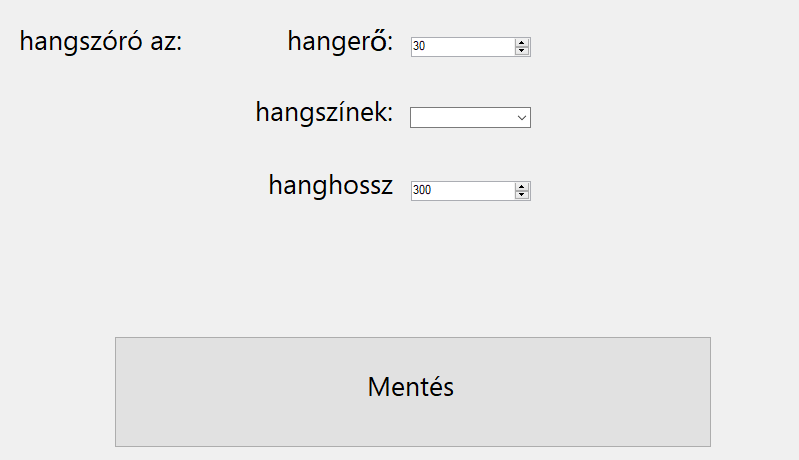
\includegraphics[page=1,width=0.5\textwidth]{hangsz_form}
	\caption[Hangszoro form]{hangszóróhoz tartozó form}
	\label{fig:hangszform}
	\end{figure}

	A hangszóró form ahogyan a nevéből is adódik a hangszóró eszköznek a szerkesztésére alkalmas képernyő ahol az adott hangszóróhoz tartozó beállításokat állíthatjuk be.
	A képernyőn megtalálhatjuk a hangszórónak az egyedi azonosítóját amely alapból egy négyjegyű hexadecimális szám amelyet a \textit{"JSON"}, szöveges formátumon keresztül, már egy ötjegyű decimális formában kerül átadásra, de mint háttéradat, hexadecimális számként tekintünk rá. A JSON-né alakítást(szerializációt) Nagy-Tóth Bence szaktársam implementálta le.
	 
	Továbbá, a képernyőn beállíthatjuk a hangerőt, hangszínt, és hanghosszt. Mindezek alap állapotban valamilyen kezdőértékkel rendelkeznek, kivéve a hangszín mezőt.
	\\
	A hangerőt lehetőség szerint maximum 63-as hangerősségig tudjuk állítani, amely természetesen az adott frekvencián kiadott hangszín hangerejét fogja beállítani.
	\\
	Ezután a hangszínt tudunk beállítani a felsorolásban található adatokból.
	\\
	Majd végül a hanghossz betudjuk állítani mindezt milliszekundumban ezért ha például 1 másodpercig szeretnénk, hogy hangozzon az adott hangszín amit megadunk az eszközünknek akkor 1000 értékre kell beállítanunk a hanghossz változót.
	\subsection{Form Lámpa Szerkesztés}
	A különböző eszközökhöz tartozó szerkesztési formokat, külön képernyő segítségével oldottuk meg, amelyek mint egyfajta \textit{"gyermek"} form-ként is szolgálnak az előző \ref{Form Szerkesztes} fejezet számára.
	\begin{figure}[h!]	
		\centering
		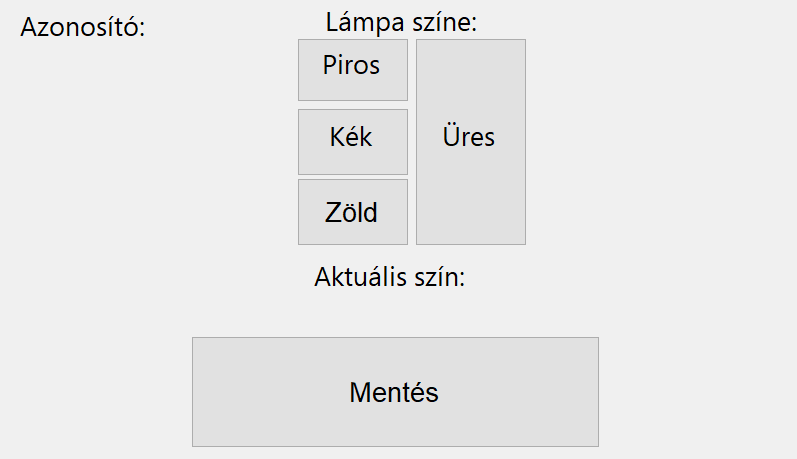
\includegraphics[page=1,width=0.5\textwidth]{lamp_form}
		\caption[Lampa form]{lámpához tartozó form}
		\label{fig:lampaform}
	\end{figure}
	A lámpa form ahogyan a fenti \ref{fig:lampaform} ábra is mutatja a géphez csatlakoztatott lámpa eszköz paramétereit konfigurálja be.
	\\
	A képernyőn megtalálható a lámpa azonosítója amely alapból egy négyjegyű hexadecimális szám amelyet a \textit{"JSON"}-ben már egy ötjegyű decimális formában kerül átadásra, de mint háttéradat hexadecimális számként tekintünk rá. Ezt a művelet Nagy-Tóth Bence szaktársam implementálta le.
	\\
	A képernyőn továbbá lehetőségünk van arra is, hogy a lámpának a színét változtassuk, piros, kék, vagy zöld színre.
	Természetesen, ki is tudjuk kapcsolni a lámpát, ekkor az \textit{"Üres"} gombbra kattintva az eszközre kimegy egy \textbf{RGB(0,0,0)} értékekkel ellátott jel.
	\\
	Az \textit{"Aktuális szín: "} címke a lámpa eszköz aktuális beállítását/színét hivatott jelezni a felhasználó számára.
	\\
	A \textit{"Mentés"} nevezetű gombbal tudjuk azt ellenőrizni, hogy a lámpánk valóban helyes jelet kap.
	
	
	\subsection{Form Nyíl Szerkesztés}
	A különböző eszközökhöz tartozó szerkesztési formokat, külön képernyő segítségével oldottuk meg, amelyek mint egyfajta \textit{"gyermek"} form-ként is szolgálnak az előző \ref{Form Szerkesztes} fejezet számára.
	
	\begin{figure}[h!]	
		\centering
		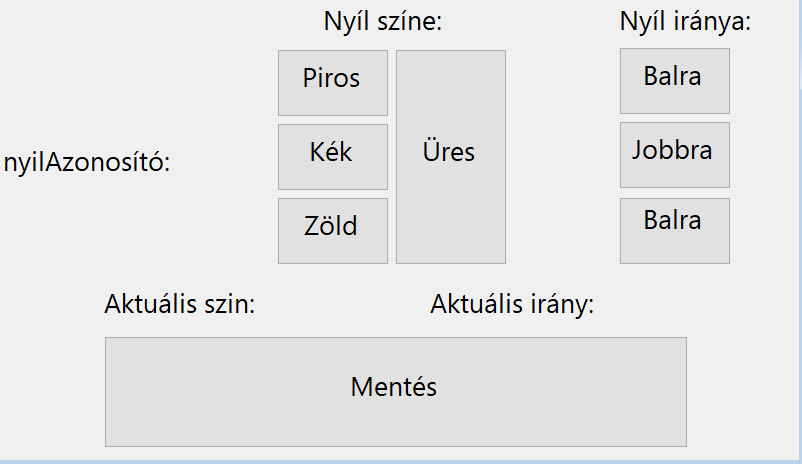
\includegraphics[page=1,width=0.5\textwidth]{nyíl_form}
		\caption[nyil form]{nyíl tartozó form}
		\label{fig:nyilform}
	\end{figure}
	A nyíl form a \ref{fig:nyilform} ábrán látható képernyőn található meg, amely képernyőt csak akkor tudunk elérni, hogyha a csatlakoztatott eszközeink közé nyíl eszköz is tartozik.
	\\
	A képernyőn megtalálható a nyílAzonosító amely alapból egy négyjegyű hexadecimális szám amelyet a \textit{"JSON"}-ben már egy ötjegyű decimális formában kerül átadásra, de mint háttéradat hexadecimális számként tekintünk rá. Ezt a művelet Nagy-Tóth Bence szaktársam implementálta le. 
	\\
	A képernyőn továbbá lehetőségünk van a nyíl színét, irányát konfigurálni. A nyíl színét háromféle színre tudjuk állítani csakúgy mint a lámpánál.
	 A színek lehetnek:
	\begin{enumerate}
		\centering
		\item Piros (RGB(255,0,0))
		\item Kék (RGB(0,0,255))
		\item Zöld (RGB(0,255,0))
	\end{enumerate} 

	A nyíl irányát is lehet változtatni, balra, jobbra, vagy akár mindkét irányba is lehetséges. Ez mindösszesen annyit jelent az eszköz számára, hogy a nyílban lévő LED-ek más és más pozícióban kapnak feszültséget.
	\\
	A nyilak ellenőrzésére a \textit{Mentés} gombot kell lenyomni, amely egy esemény hatására, a nyíl eszköznek kiküldi a megfelelő konfigurációkat .
	
	\begin{comment}
		3.fejezet(vége): kitekintés, milyen más rendszerek vannak még, és ahhoz képest ez mit tud, vannak hasonló szoftverek, vannak tréner szoftverek, de a mienk az spec képzésre alkalmas
		- szoftver és a hardvert hozzákellett fejleszteni, ez egy prototípus. Miért nem lehet ennek hasonló változata
		Még kiegészíteni valamivel.
	\end{comment}
	\chapter*{Kitekintés}
	A rendszer amit kiépítettünk, azon okból egyedülálló mivel a hardveres háttere specifikusan épül fel, és jelen állapotában az SLDLL képes vezérelni ezen eszközök helyes működését.
	\\
	Lehetséges ötletek, az eszközök felhasználására, akár az lehetne, hogy mintegy közlekedési lámpa szimulálása amely három lámpa egységes összekötéséből és vezérléséből állna. Emellett, ha megtoldanánk egy hangszóró eszközzel is akkor egy hangjelzéses, átkelő lámpát is tudnánk ezzel szimulálni.
	Mindezek az ötletek jelenlegi projektnek nem képezik szerves részét, de jövőbeni használatra, és továbbfejlesztésre, mindenképpen alkalmas lehet.
	\begin{comment}
		4.fejezet: (future works) továbbiakban milyen kimenetele lesz, ebből szabadalom lesz, az ötletgazda szeretné ezt kiadni olyan módon hogy piaci termék legyen. 
		- Teljesen más technológia
	\end{comment}
	
	\begin{comment}
		5.fejezet:  összefoglaló, melyik fejezetben miről beszéltünk, miket sikerült elérni(pl 1.fejezetben említetteket megcsináltam, iylenek), Mi az EREDMÉNY! miért fontos, 
		- miért jó ez? Működés közben videókat kéne csinálni. Érdemes lenne titkosítani.
	\end{comment}
	\chapter*{Végkitekintés}
	Jelenlegi projekt során, ablakos applikációt tudtunk készíteni amely segítségével három fajta eszközt tudunk vezérelni akár önállóan egy eszközt, vagy együttesen 2 vagy 3 eszközt.

	Nagyon örültünk, hogy egy kis betekintést nyerhettünk az egészségfejlesztés világába, Somodi László gondolatain keresztül amelyet a vele való beszélgetéseinkből, valamint \textit{,,Mozgáskoordináció- és gyorsaságfejlesztő gyakorlatok óvodától a felnőtt korig''} című alkotásában leírt gondolatokból szereztük.
	
	Személy szerint kíváncsisággal töltött el az a gondolat, hogy az informatikával mint olyannal képesek vagyunk segíteni felebarátainkon legjobb tudásunk szerint, amellyel az Isten megáldott bennünket.
	
	Örömömre szolgált, hogy Somodi László minket bízott meg elméleteit kivitelező szoftveres háttérrel. Szakdolgozatunk nem csupán arról szól, hogy amit megtanultunk a gyakorlatban azt kamatoztassuk, és bizonyítsunk másoknak, hanem ezzel a projekttel sok olyan ember számára tudunk további segítséget nyújtani akik rászorulnak az ilyesfajta segítségre.
	
	Munkánkat több tudományág összehangolt kutatómunkája segítette elő, ezen okból kifolyólag szerteágazónak is nevezhetnénk a projekt összeállítását.
	
	Ami a programozási elméletet és ennek gyakorlati vonatkozásait illeti, Dr. Király Roland Tanár Úr segített bennünket, a projekt elindulásában, mivel, hogy annak idején ő tervezte az alapprogramnak a felépítését és struktúráját. Emellett, konzultációk során is segített gondolatokat nyerni és ezeket a program szerves részévé tenni.

\verb*|#TODO|: Saját kitekintés mik vannak ilyen hasonlók
	
	\begin{comment}
		Mint minden szoftverre és emberi termékre jellemző, a megoldásaink természetesen nem mondhatóak tökéletesnek, programunk épp annyira időnként karbantartásra és további fejlesztésekre szorulhat. Érdekes volt felfedezni a gRPC és a Proto-nyelv kapcsán a \ref{grpc} fejezetben, hogy ötször-hatszor jobb teljesítmény érhető el az adatok bináris módon történő szerializációjával a szöveges formátumokhoz képest -- jelen állás szerint mégis az utóbbi megoldás számít elterjedtebbnek --, én azt gondolom, hogy mindenképp érdemes lenne munkánkat esetleg egy másik szakdolgozat keretein belül a gRPC irányába elmozdítani.
	\end{comment}

	\chapter*{Köszönetnyílvánítás}
	Szeretném köszönetemet ezúton is kifejezni a konzulensemnek, Dr.Király Roland Tanár Úrnak, aki lehetővé tette ezen téma feldolgozását.
	Továbbá, szeretném megköszönni, kedves barátomnak és szaktársamnak, Nagy-Tóth Bencének a sok fáradságos munkáját, amely alapját képezte a programomnak. 
	\\
	Végső soron, Istennek szeretném hálámat kifejezni, mivel a tudásomat és a kitartásomat, Tőle nyerhetem mindennap. 
	

	

	\bibliographystyle{plain}
	\bibliography{references}
	\begin{comment}
		1.Alapötlet, Projekt célja, és hatásai az oktatásra/egézségügyre.
				Miért jó a projekt amit csinálunk?
				Somodi László által kapottak megemlítése
		2.A Winformos projekt
				milyen eszközöket lehet irányítani vele(mire jók)
				panelek külön-külön mit csinálnak
				hogyan kommunikál a Delphi-vel (Bence projektje, megemlítés)
		3. Alacsonyabbszintű komponensek/Imperatív és oop közti kommunikáció(Bence)
				Hangvezérlés
				Színek
				Nyilak
				4 || 8 eszközös megoldások
		4. Projekt tényleges használata, felmérések, és vélemények.
				Gondolatok és meglátások //akár lehet egyel előbb is
	\end{comment}
	% Aláírt, szkennelt nyilatkozat beillesztése a szakdolgozat végére
	%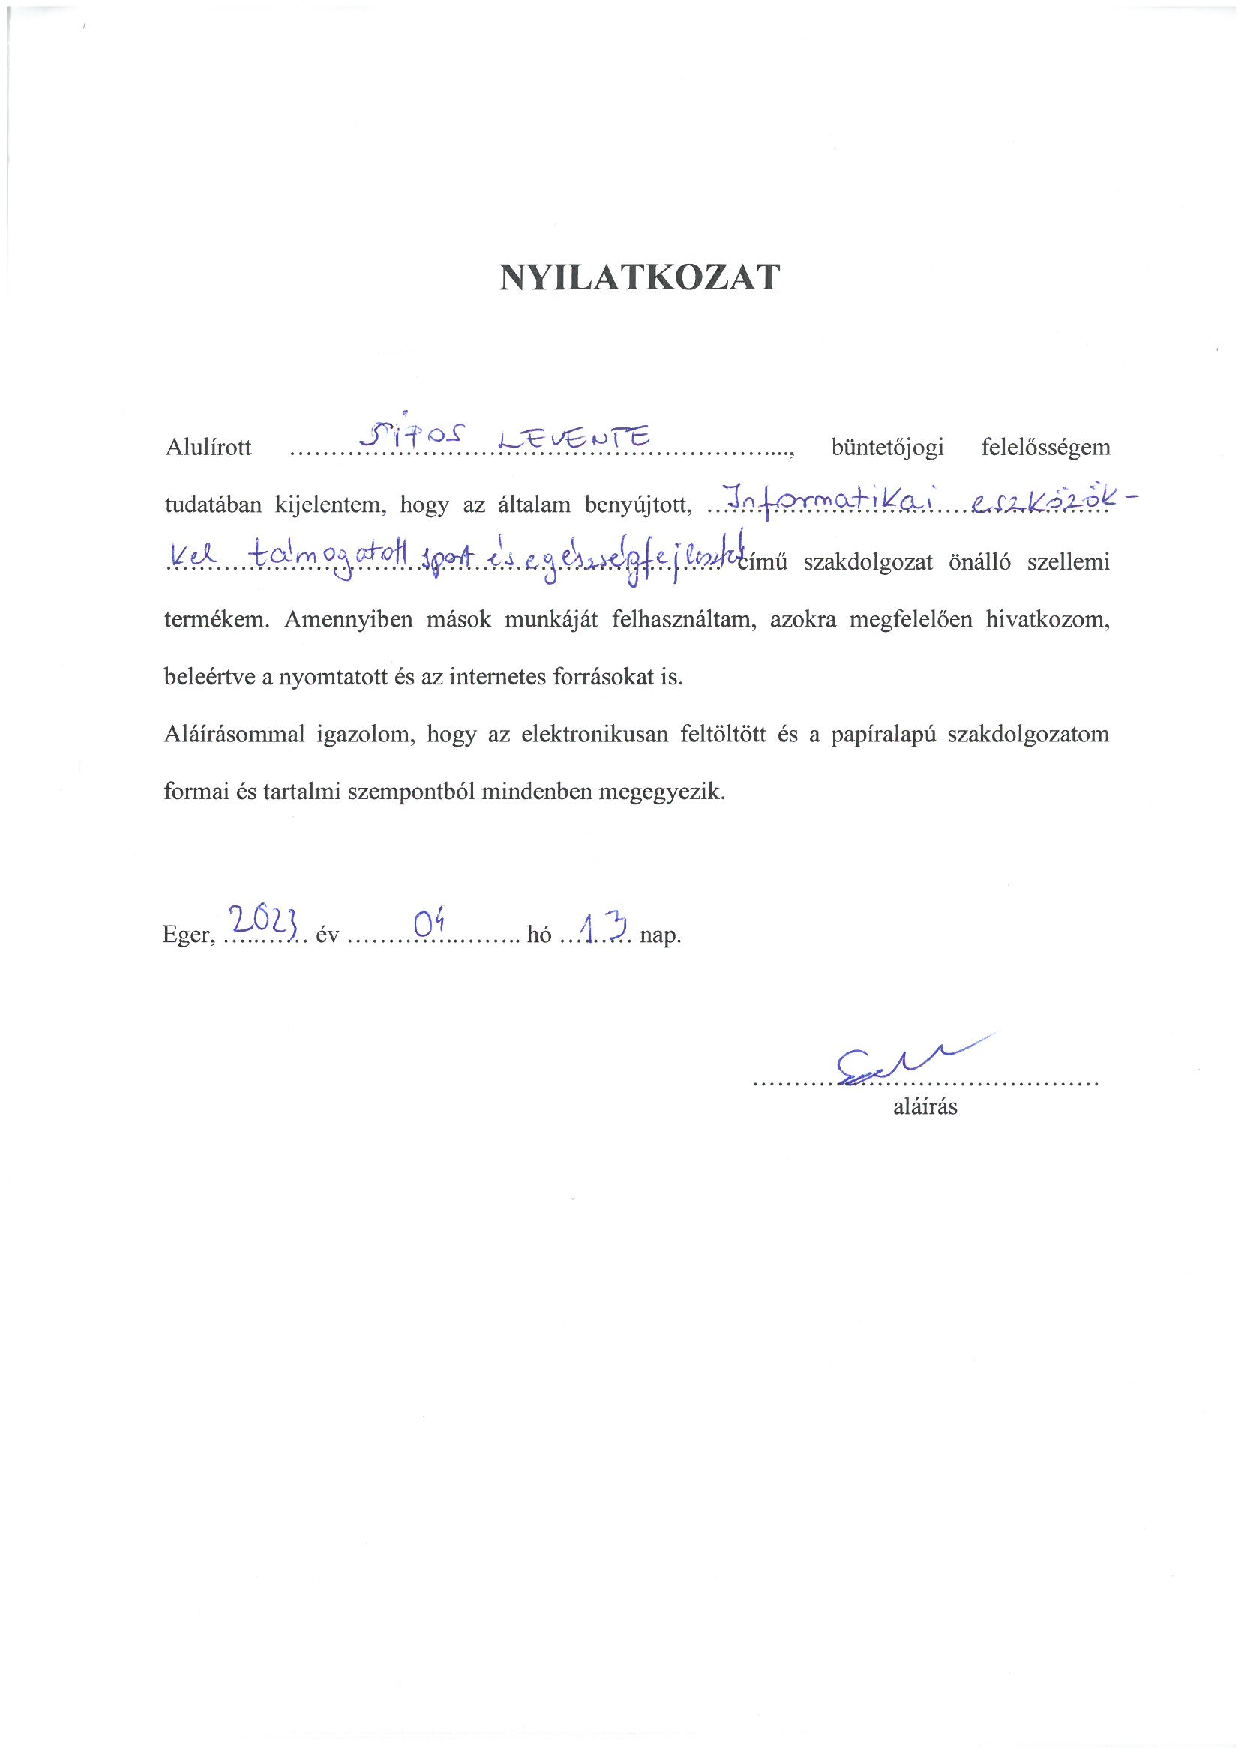
\includepdf{nyilatkozat.pdf}
	\listoffigures
\end{document}